\documentclass[10pt]{beamer}

\newcommand{\lectnum}{L02}
\newcommand{\lecttitle}{AI For X: A Landscape Tour}

\usepackage{amsmath, amssymb, graphicx}
\usepackage[]{algorithm2e}
\usepackage{pdfpages}
\usepackage{bm}
\usepackage{relsize}
\usepackage[british]{babel}
\usepackage{tikz,tikzsymbols}
\usepackage{hyperref}
\usepackage{cancel}
\usepackage{caption,subcaption}
\usepackage{adjustbox}
\usepackage{overpic}
\usepackage[UKenglish]{isodate}
\usepackage{tabularx}
\usepackage{array}
\usepackage{booktabs}

\usetikzlibrary{arrows,decorations.markings,positioning,calc,shapes.multipart}

\newcommand{\bs}{\boldsymbol}


\hypersetup{colorlinks,linkcolor=,urlcolor=blue}
\newenvironment{titledslide}[1]{\begin{frame}\frametitle{#1}}{\end{frame}}

\mode<presentation>{\setbeamercovered{transparent}}

\setbeamertemplate{sidebar right}{}
\setbeamertemplate{footline}{%
\hfill\usebeamertemplate***{navigation symbols}
\hspace{0.4cm}\lectnum: \insertframenumber{}/\inserttotalframenumber \hspace*{0.4cm}}

\author{Mengyan Zhang}

\title{COMS20018, Introduction to AI:\\ \vspace{5pt} \lecttitle}

\institute{School of Computer Science\\University of Bristol}
\date{21st September 2026}

%%%%%%%%%%%%%%%%%%%%%%%%%%%%%%%%%%%%%%%%%%%%%%%%%%%%%%%%%%%%%%%%%%%%%%

\begin{document}
%%%%%%%%%%%%%%%%%%%%%%%%%%%%%%%%%%%%%%%%%%%%%%%%%%%%%%%%%%%%%%%%%%%%%%

\begin{frame}[fragile]
  \begin{tikzpicture}[remember picture, overlay]
    \node[anchor=north west, xshift=0.4cm, yshift=-0.4cm] at (current page.north west)
      {
\includegraphics[width=3.4cm]{figs/uob_logo.png}};
  \end{tikzpicture}
  \titlepage
\end{frame}
%%%%%%%%%%%%%%%%%%%%%%%%%%%%%%%%%%%%%%%%%%%%%%%%%%%%%%%%%%%%%%%%%%%%%%
\begin{frame}[fragile]
\frametitle{The Landscape of AI Applications}

\begin{center}
\resizebox{0.98\textwidth}{!}{%
\begin{tabular}{ccccc}
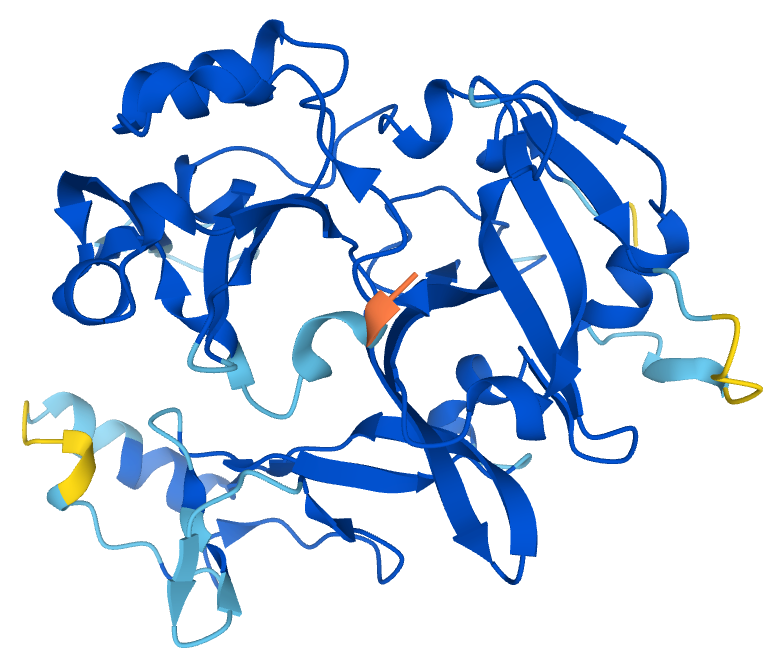
\includegraphics[height=2.1cm]{figs/protein.png} &
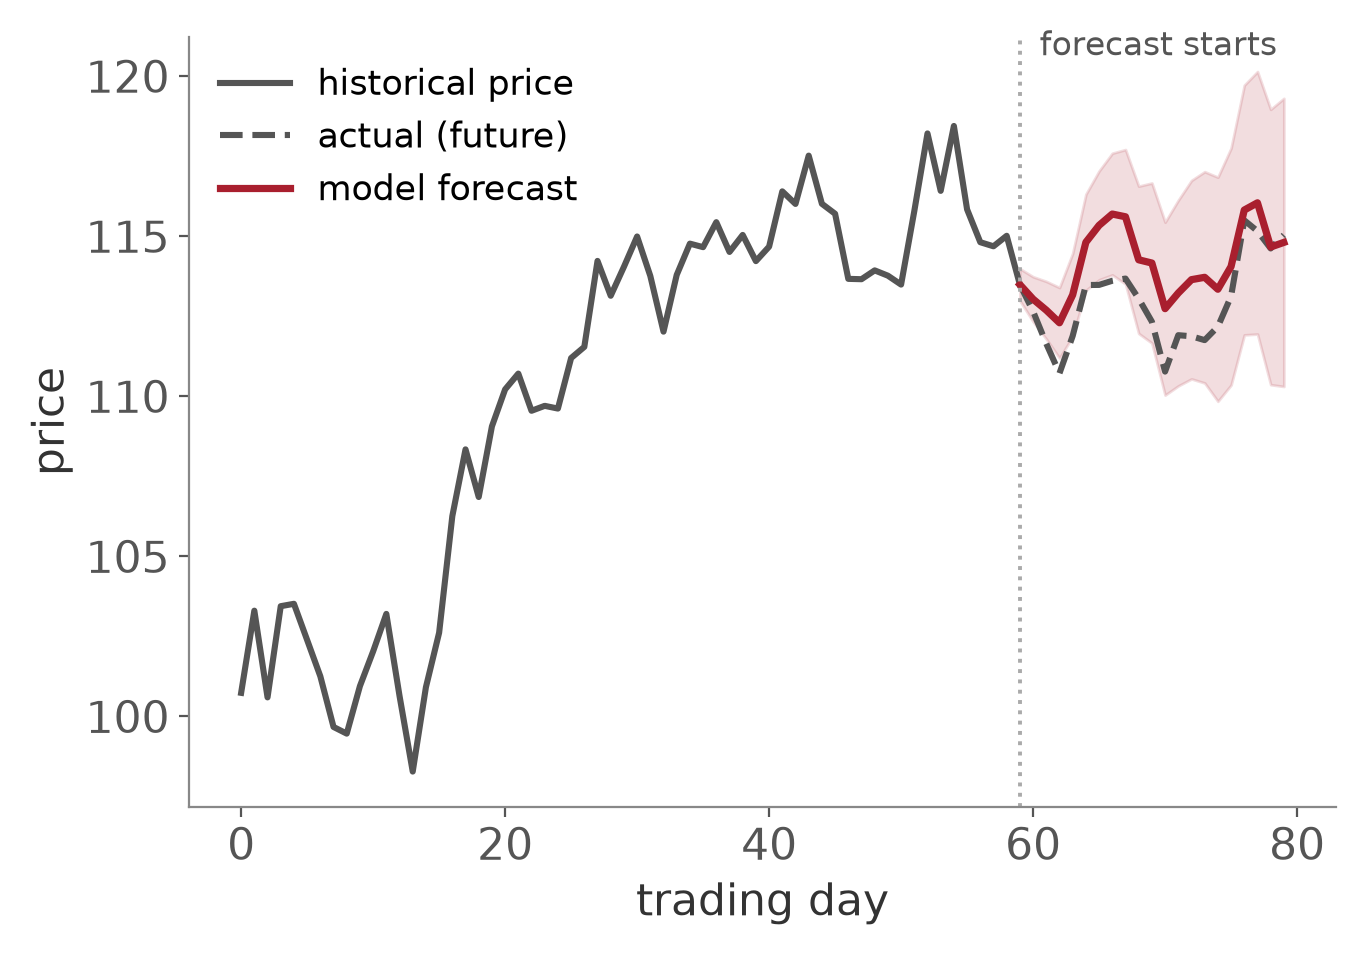
\includegraphics[height=2.1cm]{figs/finance_chart.png} &
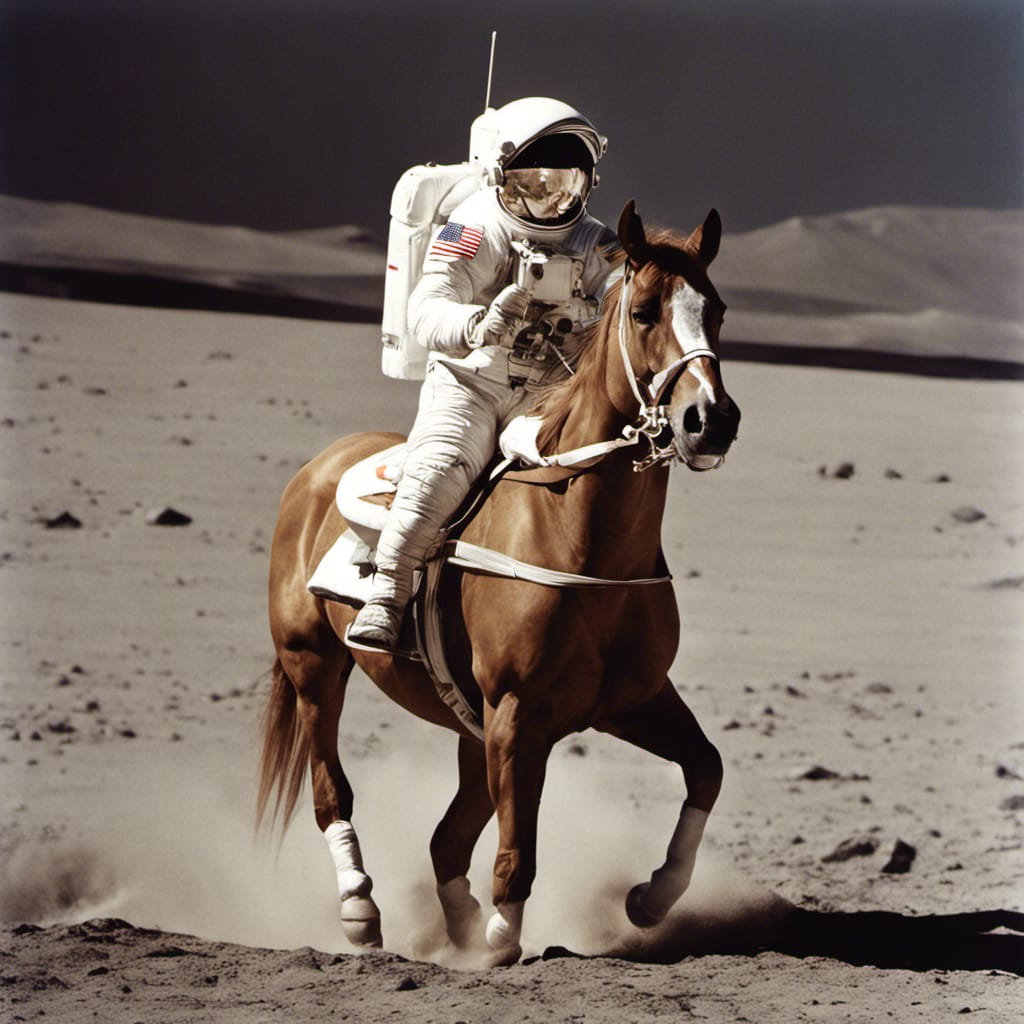
\includegraphics[height=2.1cm]{figs/genai.jpg} &

\includegraphics[height=2.1cm]{figs/tiktok_phone.png} &
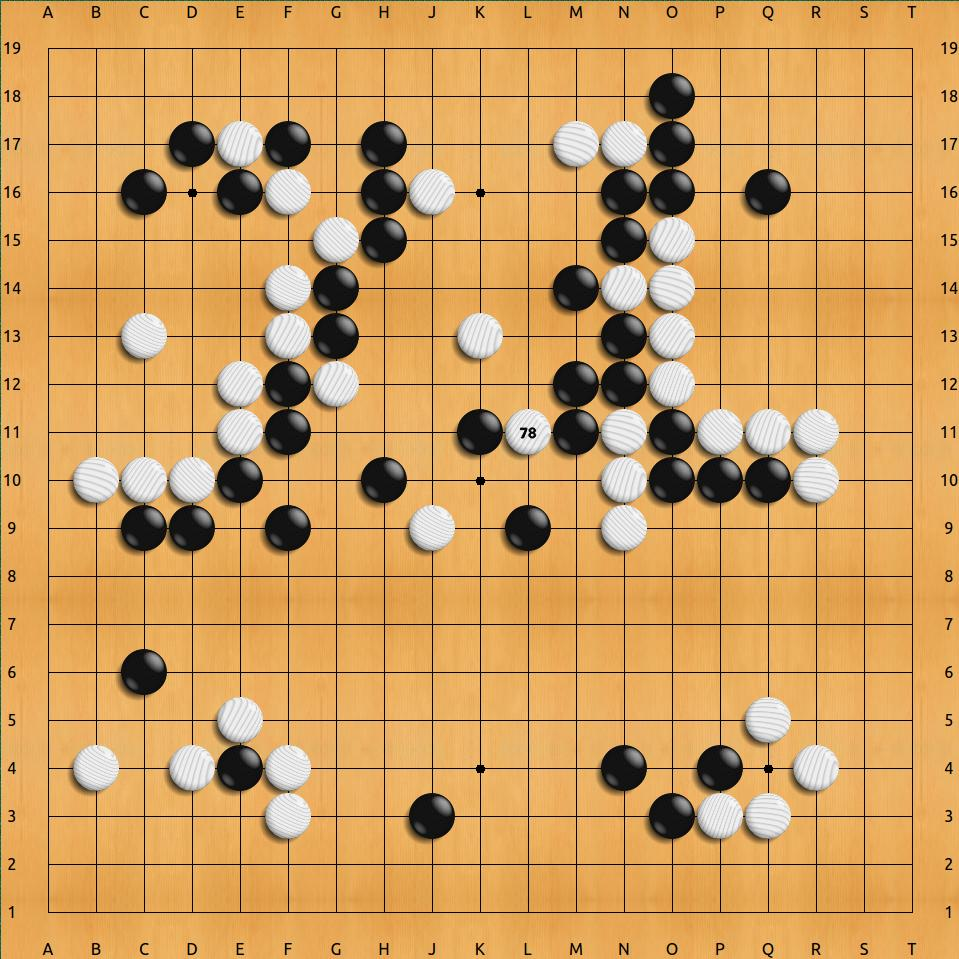
\includegraphics[height=2.1cm]{figs/alphago.jpg} \\
{\small Science} & {\small Finance} & {\small Generative AI} &
{\small Recommenders} & {\small Game playing} \\[8pt]
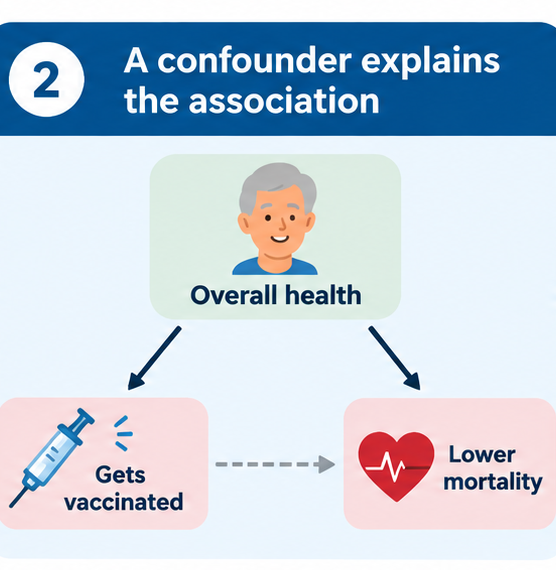
\includegraphics[height=2.1cm]{figs/causal_middle.png} &
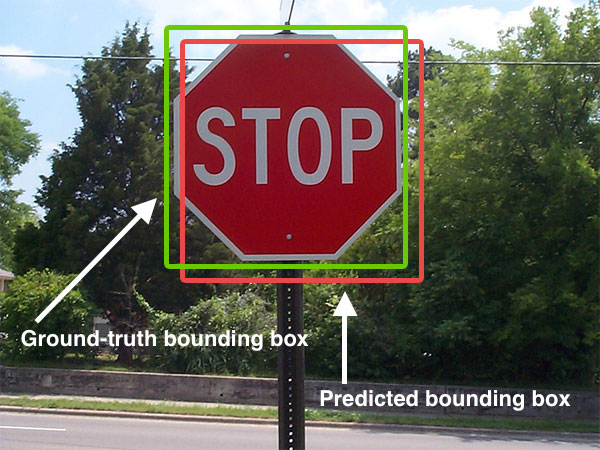
\includegraphics[height=2.1cm]{figs/cv_detection.jpg} &
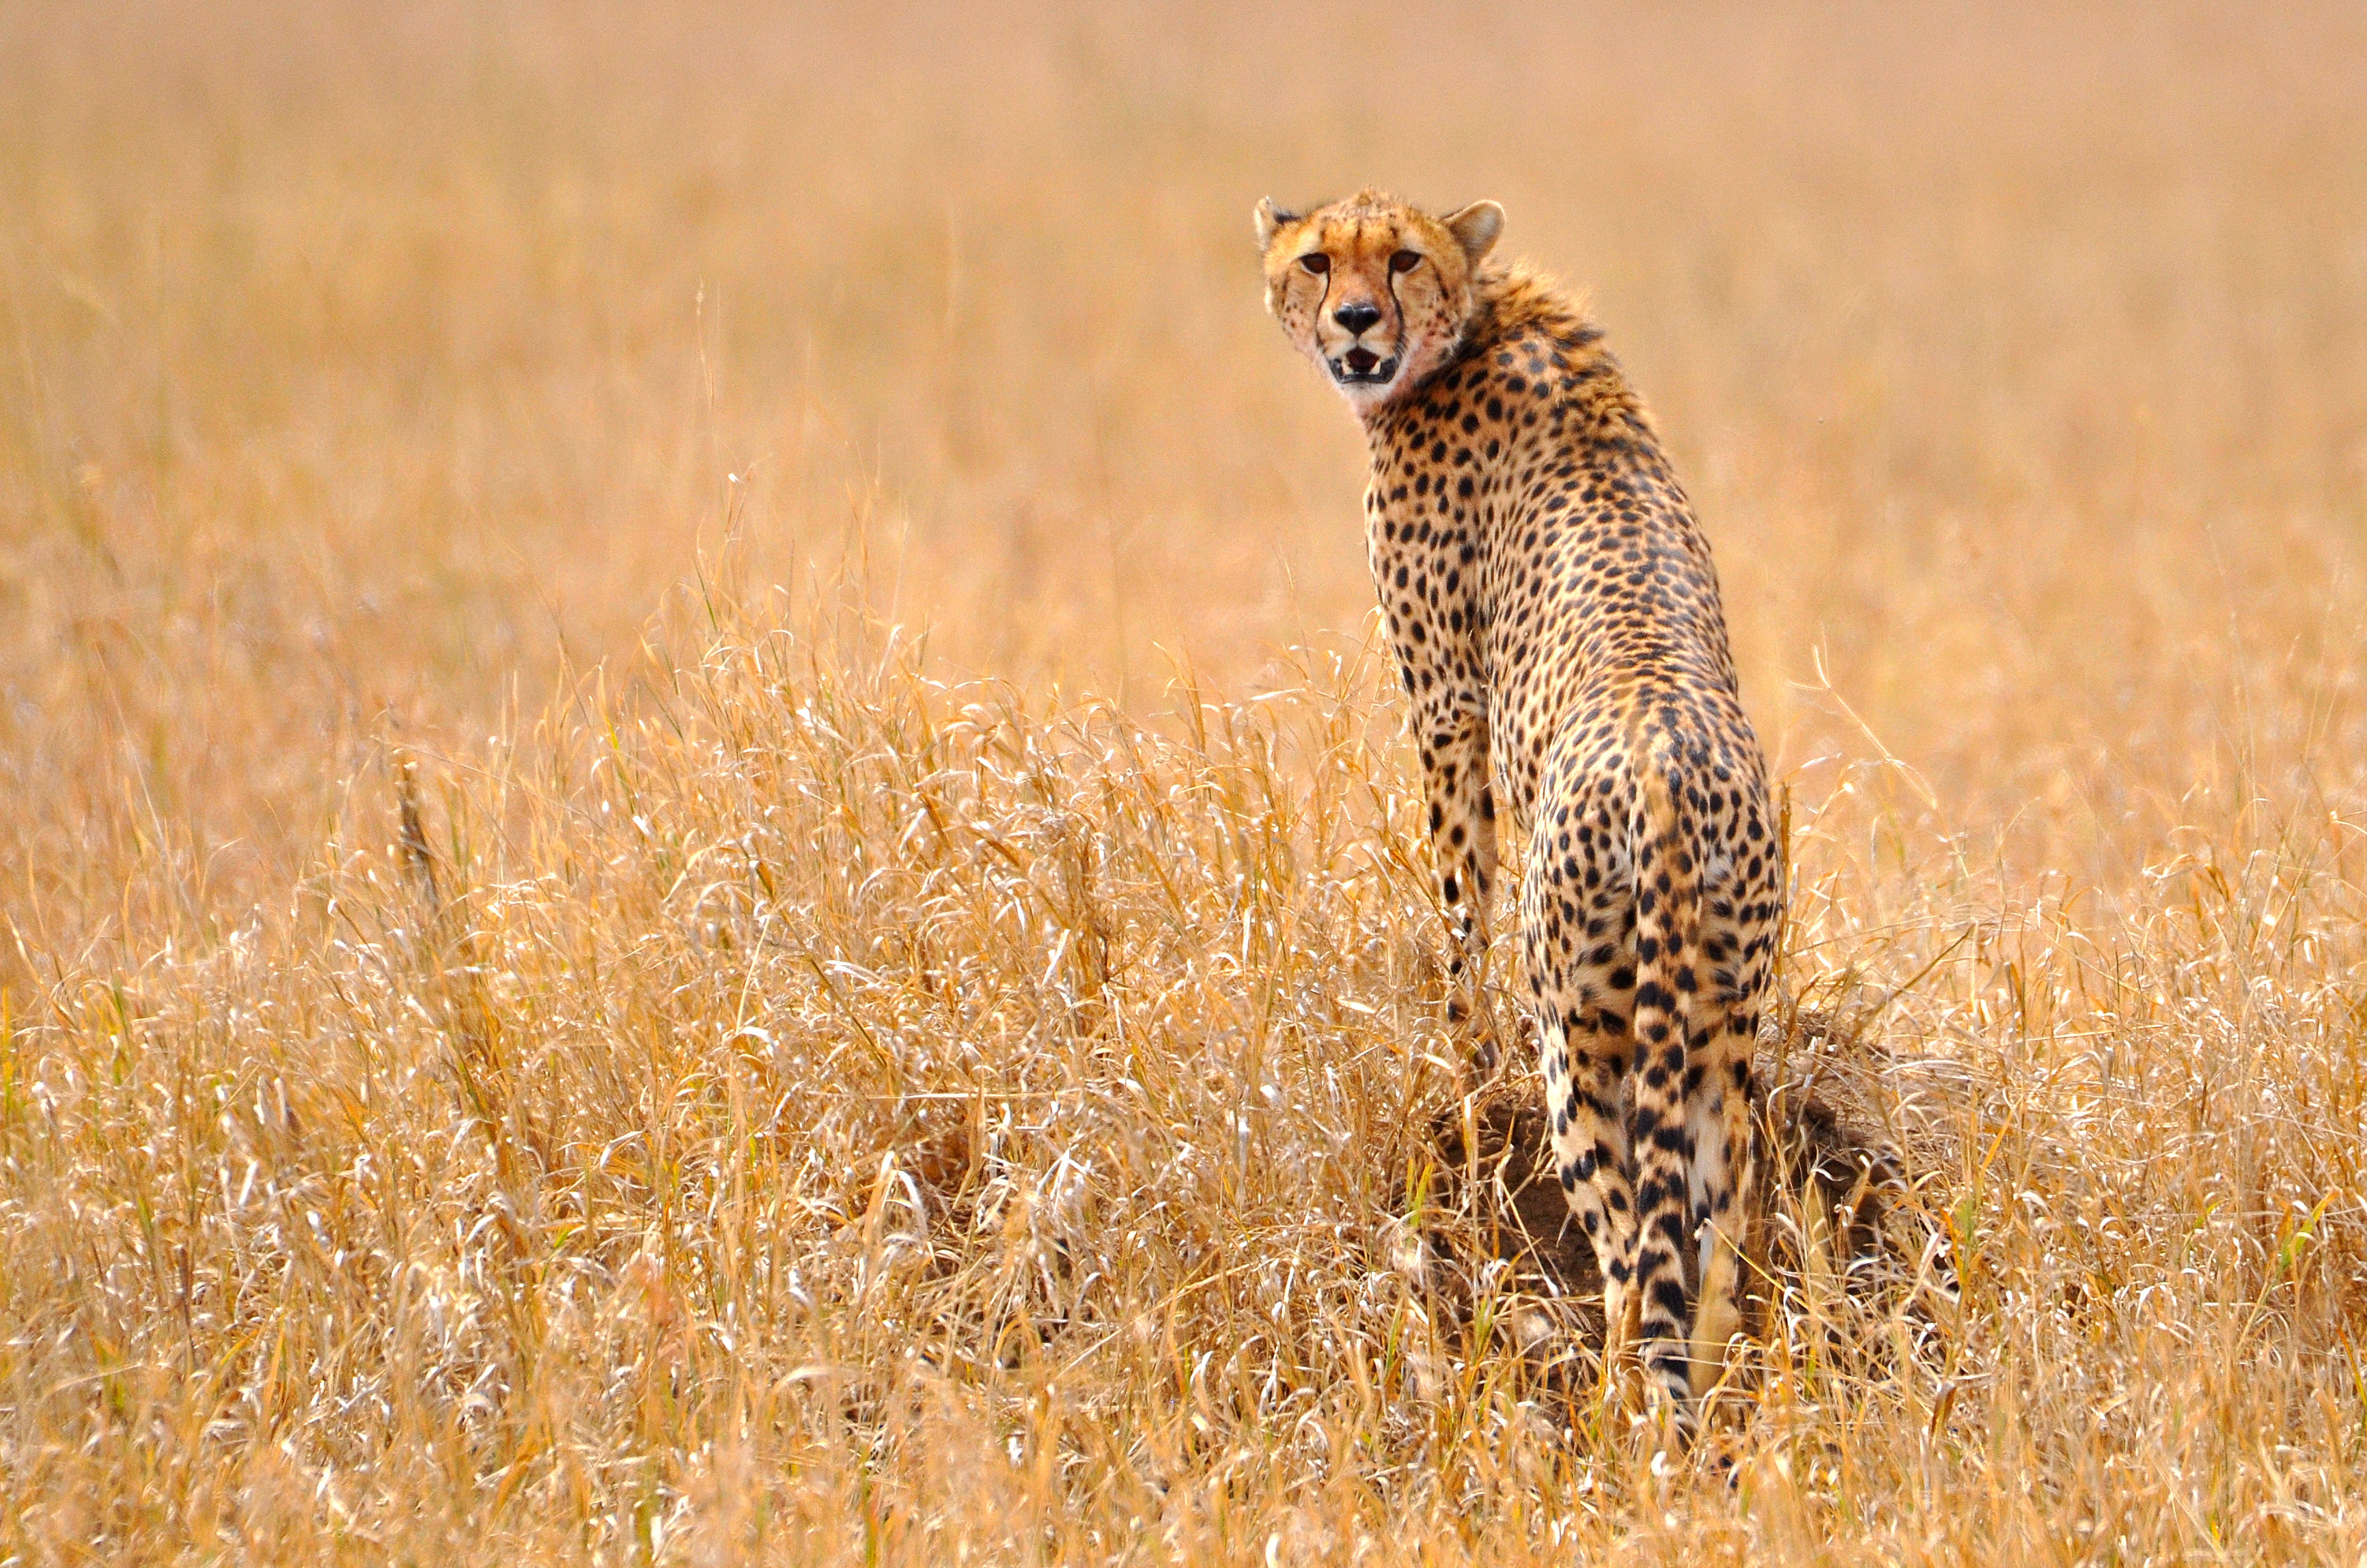
\includegraphics[height=2.1cm]{figs/wildlife.jpg} &
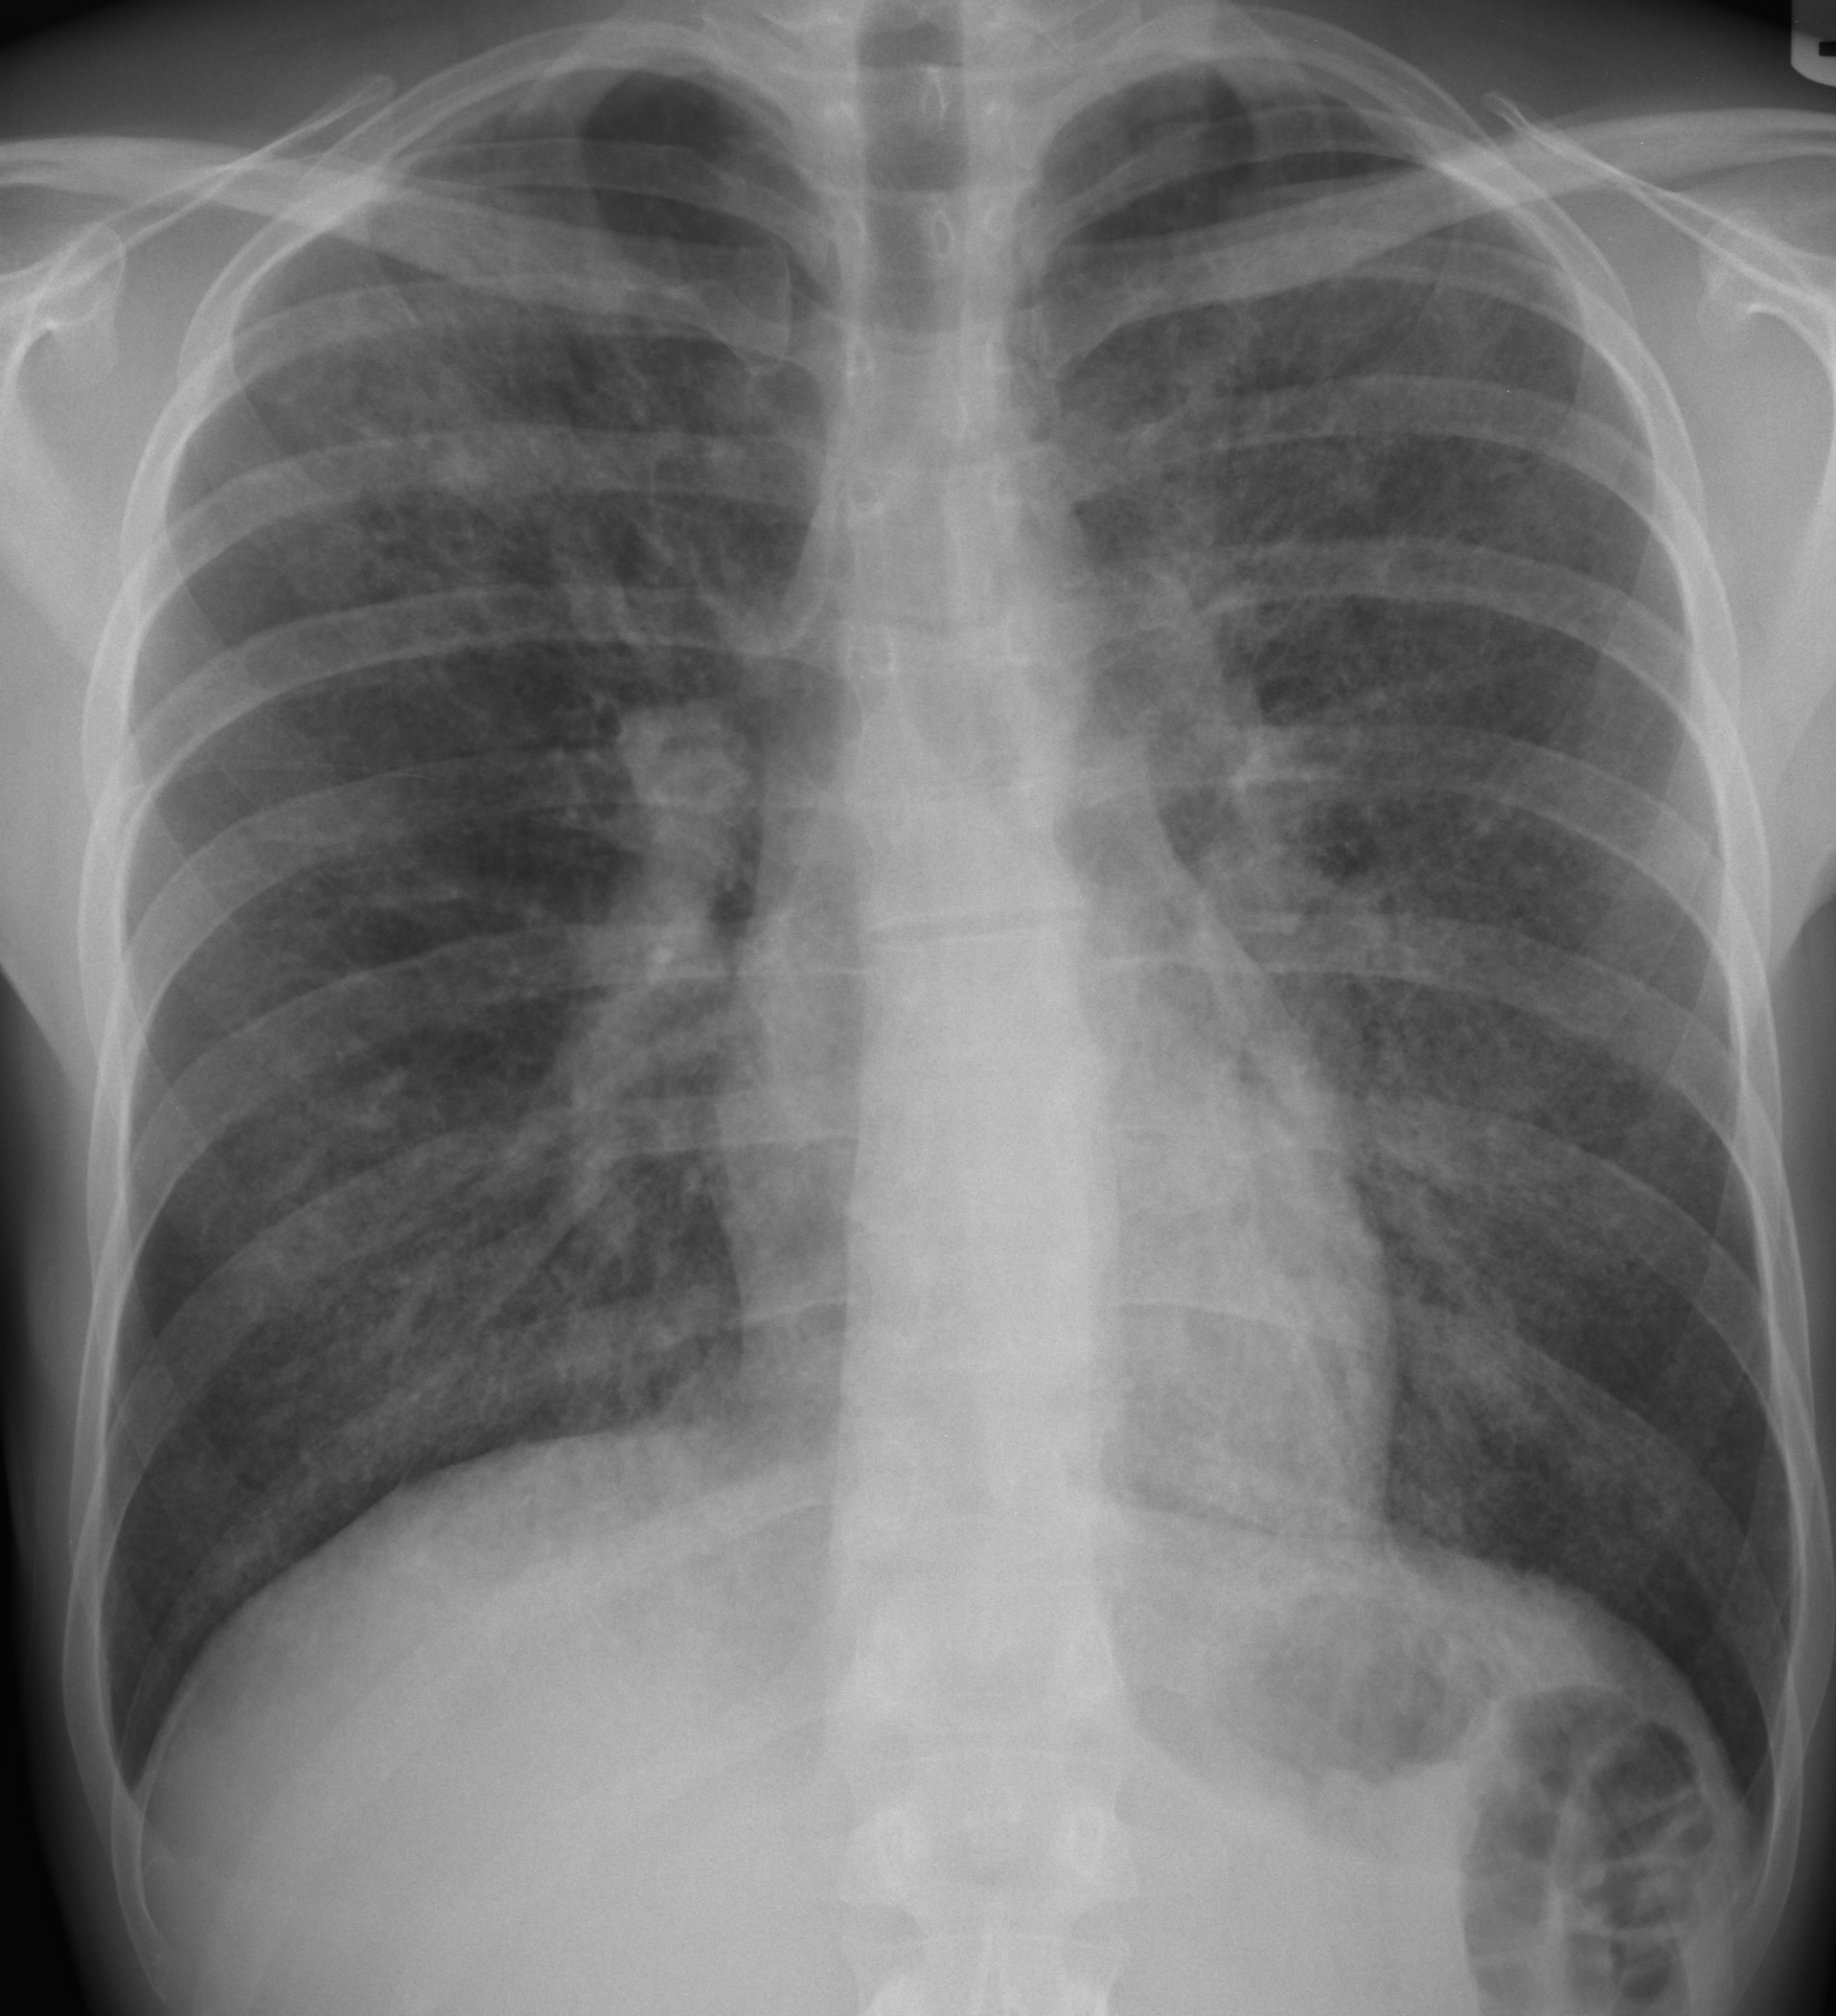
\includegraphics[height=2.1cm]{figs/healthcare_xray.jpg} &

\includegraphics[height=0.9cm]{figs/tool_logo1.png} \\
{\small Epidemiology} & {\small Computer vision} & {\small Conservation} &
{\small Healthcare} & {\small Everyday AI tools}
\end{tabular}}
\end{center}

\vspace{10pt}
\begin{itemize}
\item[$\Rightarrow$] A quick tour of where AI already shows up around
  you, then how this unit gets you there.
\end{itemize}

\end{frame}
%%%%%%%%%%%%%%%%%%%%%%%%%%%%%%%%%%%%%%%%%%%%%%%%%%%%%%%%%%%%%%%%%%%%%%
\begin{frame}[fragile]
\frametitle{Solving a 50-Year-Old Problem in Biology}
\framesubtitle{AI for X \textperiodcentered\ Science}

\begin{columns}[T]
\begin{column}{0.45\textwidth}
\centerline{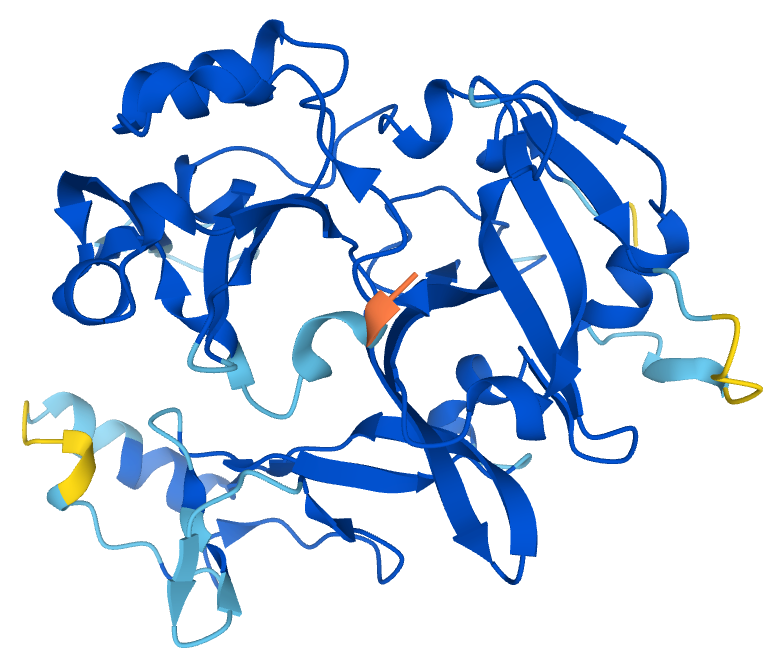
\includegraphics[width=\textwidth]{figs/protein.png}}
\end{column}
\begin{column}{0.53\textwidth}
\begin{itemize}
\item The ``protein folding problem'': predict a protein's 3D shape from
  its amino-acid sequence
\item AlphaFold 2 (DeepMind) predicts structures at near-experimental
  accuracy for most proteins
\item \textbf{Under the hood:} a deep neural network trained on
  \textasciitilde170,000 known structures 
\item 200+ million structures released freely; won the 2024 Nobel
  Prize in Chemistry
\end{itemize}
\end{column}
\end{columns}

\vspace{8pt}
{\footnotesize Image: human C12orf29 protein structure predicted by
AlphaFold. CSBIOPASSION, Wikimedia Commons, CC BY-SA 4.0. Method: Jumper
et al., \emph{Nature} (2021).}

\end{frame}
%%%%%%%%%%%%%%%%%%%%%%%%%%%%%%%%%%%%%%%%%%%%%%%%%%%%%%%%%%%%%%%%%%%%%%
\begin{frame}[fragile]
\frametitle{Can a Model Predict Tomorrow's Price?}
\framesubtitle{AI for X \textperiodcentered\ Quantitative Finance}

\begin{columns}[T]
\begin{column}{0.5\textwidth}
\centerline{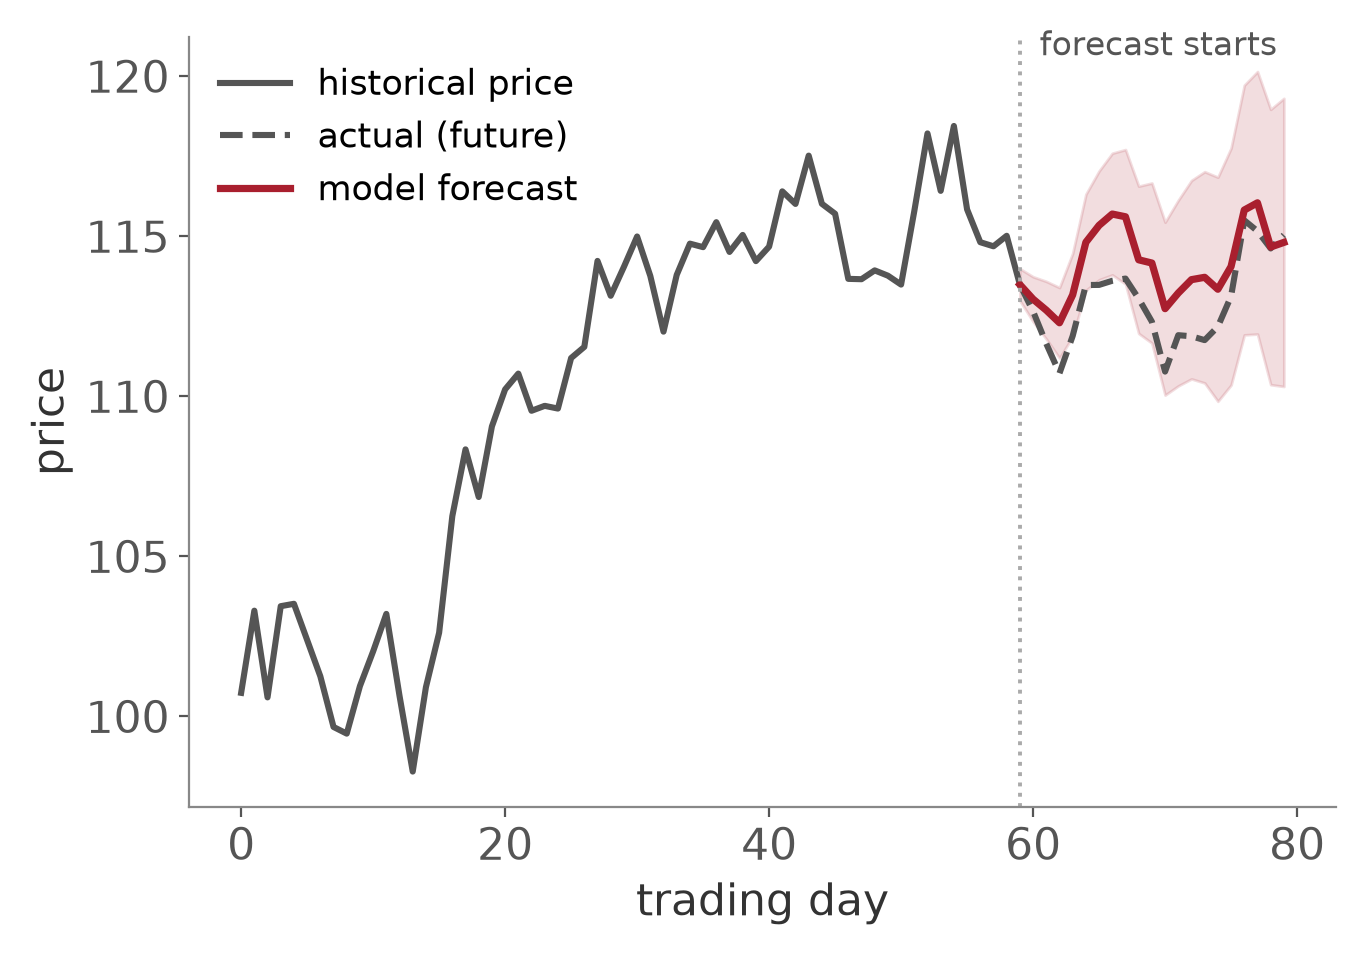
\includegraphics[width=\textwidth]{figs/finance_chart.png}}
\end{column}
\begin{column}{0.48\textwidth}
\begin{itemize}
\item Task: forecast a price (or a return) from historical patterns and
  market signals
\item \textbf{Under the hood:} regression and recurrent/transformer
  models trained on historical time series
\item The shaded band matters as much as the line; markets are noisy,
  so a good forecast reports uncertainty
\end{itemize}
\end{column}
\end{columns}

\end{frame}
%%%%%%%%%%%%%%%%%%%%%%%%%%%%%%%%%%%%%%%%%%%%%%%%%%%%%%%%%%%%%%%%%%%%%%
\begin{frame}[fragile]
\frametitle{Machines That Create: Images, Music, and More}
\framesubtitle{AI for X \textperiodcentered\ Generative Models}

\begin{columns}[T]
\begin{column}{0.42\textwidth}
\centerline{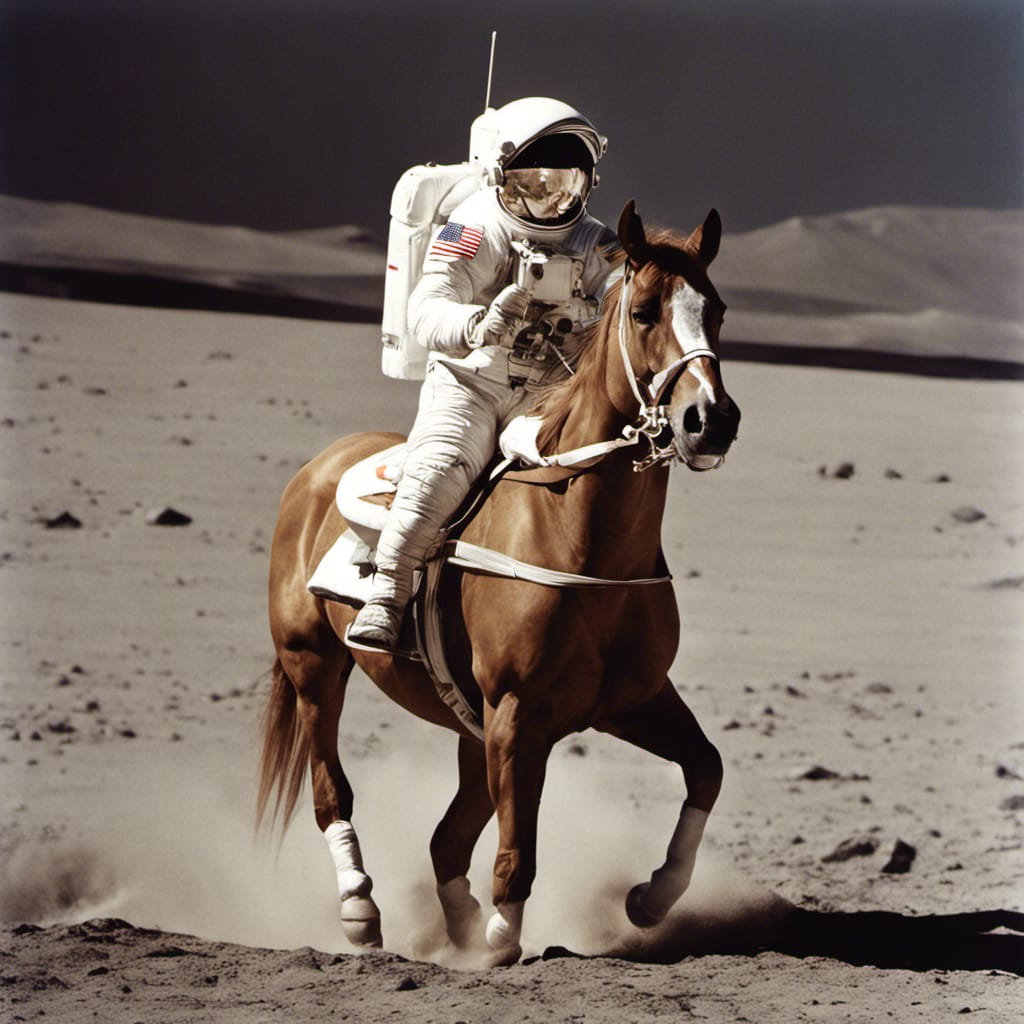
\includegraphics[width=\textwidth]{figs/genai.jpg}}
\end{column}
\begin{column}{0.56\textwidth}
\begin{itemize}
\item ``An astronaut riding a horse''; text prompt in, brand-new image
  out
\item \textbf{Under the hood:} diffusion models start from pure noise and
  repeatedly refine it toward a coherent image, guided by the text prompt
\item The same idea generates music (Suno, Udio) and video (Sora), not
  just images
\item You'll meet generative models in Week 3
\end{itemize}
\end{column}
\end{columns}

\vspace{8pt}
{\footnotesize Image: ``Astronaut Riding a Horse'', generated with Stable
Diffusion XL. VulcanSphere, Wikimedia Commons, CC0 / public domain.}

\end{frame}
%%%%%%%%%%%%%%%%%%%%%%%%%%%%%%%%%%%%%%%%%%%%%%%%%%%%%%%%%%%%%%%%%%%%%%
\begin{frame}[fragile]
\frametitle{AI Tools You Already Use}
\framesubtitle{AI for X \textperiodcentered\ Everyday tools}

\centerline{
\begin{tabular}{cccc}

\includegraphics[width=0.22\textwidth]{figs/tool_logo1.png} &

\includegraphics[width=0.22\textwidth]{figs/tool_logo2.png} &

\includegraphics[width=0.22\textwidth]{figs/tool_logo3.png} &

\includegraphics[width=0.22\textwidth]{figs/tool_logo4.png}
\end{tabular}}

\vspace{10pt}
\begin{itemize}
\item These are large language models (LLMs): transformer neural networks
  with billions of parameters
\item Trained in two stages:
  \begin{itemize}
  \item self-supervised pretraining on huge amounts of text, predict the
    next word
  \item fine-tuning with human feedback (RLHF) to be helpful, honest, and
    safe
  \end{itemize}
\item You'll learn the Transformer and LLM behind these in Week 3 and 4
\end{itemize}

\vspace{8pt}
% {\footnotesize Logos are trademarks of their respective owners (OpenAI,
% Anthropic, Google, Microsoft), shown here for identification only.}

\end{frame}
%%%%%%%%%%%%%%%%%%%%%%%%%%%%%%%%%%%%%%%%%%%%%%%%%%%%%%%%%%%%%%%%%%%%%%
\begin{frame}[fragile]
\frametitle{Can AI Ever Be Conscious?}
\framesubtitle{AI for X \textperiodcentered\ Philosophy of AI}

\begin{itemize}
\item LLMs write fluently, hold conversations, and sometimes claim to
  have feelings; does that mean anything is actually happening
  ``inside''?
\item A live scientific and philosophical debate, not one that better
  benchmarks alone will settle
% \item \textbf{One argument:} AI, psychology and philosophy often debate
%   consciousness while ignoring \emph{embodiment}, it may take a body,
%   not just a brain (or a network), to be conscious
% \item[$\Rightarrow$] We won't resolve this today; Week 5 (Philosophy
  % of AI) is where we dig into questions like this properly
\end{itemize}

\vspace{8pt}
{\footnotesize Birhane, A. ``Can AI ever be conscious? The question
stems from a misconception.'' \emph{Nature}, 656 (2026).
\url{https://www.nature.com/articles/d41586-026-02571-9}}

\end{frame}
%%%%%%%%%%%%%%%%%%%%%%%%%%%%%%%%%%%%%%%%%%%%%%%%%%%%%%%%%%%%%%%%%%%%%%
% \begin{frame}[fragile]
% \frametitle{Turning Words Into Numbers}
% \framesubtitle{AI for X \textperiodcentered\ Natural Language Processing}

% \begin{columns}[T]
% \begin{column}{0.48\textwidth}
% \centerline{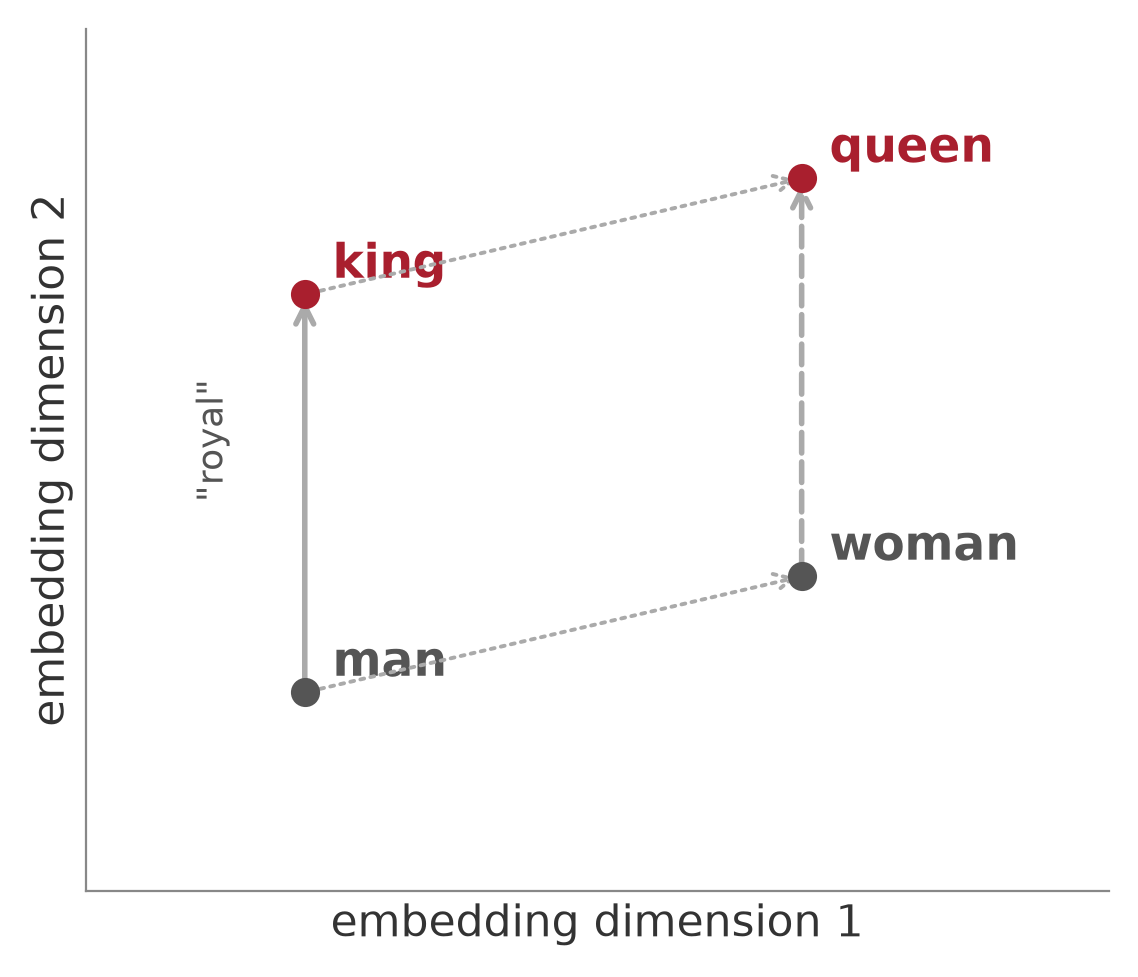
\includegraphics[width=\textwidth]{figs/nlp_embeddings.png}}
% \end{column}
% \begin{column}{0.5\textwidth}
% \begin{itemize}
% \item Words become vectors (``embeddings''); similar meanings sit close
%   together in space
% \item Vector arithmetic captures relationships:
%   \begin{itemize}
%   \item $\text{king} - \text{man} + \text{woman} \approx \text{queen}$
%   \end{itemize}
% \item Modern NLP is built on Transformers (Week 4), the same
%   architecture behind ChatGPT and Claude
% \item Applications: translation, summarisation, search, sentiment
%   analysis
% \end{itemize}
% \end{column}
% \end{columns}

% \vspace{8pt}
% {\footnotesize Illustration inspired by the classic word2vec analogy
% result of Mikolov et al.\ (2013).}

% \end{frame}
%%%%%%%%%%%%%%%%%%%%%%%%%%%%%%%%%%%%%%%%%%%%%%%%%%%%%%%%%%%%%%%%%%%%%%
\begin{frame}[fragile]
\frametitle{How TikTok Decides What's Next}
\framesubtitle{AI for X \textperiodcentered\ Recommender Systems}

\begin{columns}[T]
\begin{column}{0.33\textwidth}
\centerline{
\includegraphics[width=0.85\textwidth]{figs/tiktok_phone.png}}
\end{column}
\begin{column}{0.63\textwidth}
\begin{itemize}
\item Task: predict which video you'll watch (and for how long), from
  your past behaviour
\item \textbf{Signals used:} watch time, likes, comments, shares, feed a
  ranking model that scores every candidate video for you
\item \textbf{Under the hood:} deep learning embeddings of users and
  videos, updated continuously as you interact, a modern descendant of
  matrix factorisation
\end{itemize}
\end{column}
\end{columns}

\vspace{8pt}
{\footnotesize See TikTok's public ``How TikTok
recommends videos'' (2020).}

\end{frame}
%%%%%%%%%%%%%%%%%%%%%%%%%%%%%%%%%%%%%%%%%%%%%%%%%%%%%%%%%%%%%%%%%%%%%%
\begin{frame}[fragile]
\frametitle{Biased Recommendation and Exploration}
\framesubtitle{AI for X \textperiodcentered\ Ethics \& Reinforcement Learning}

\centerline{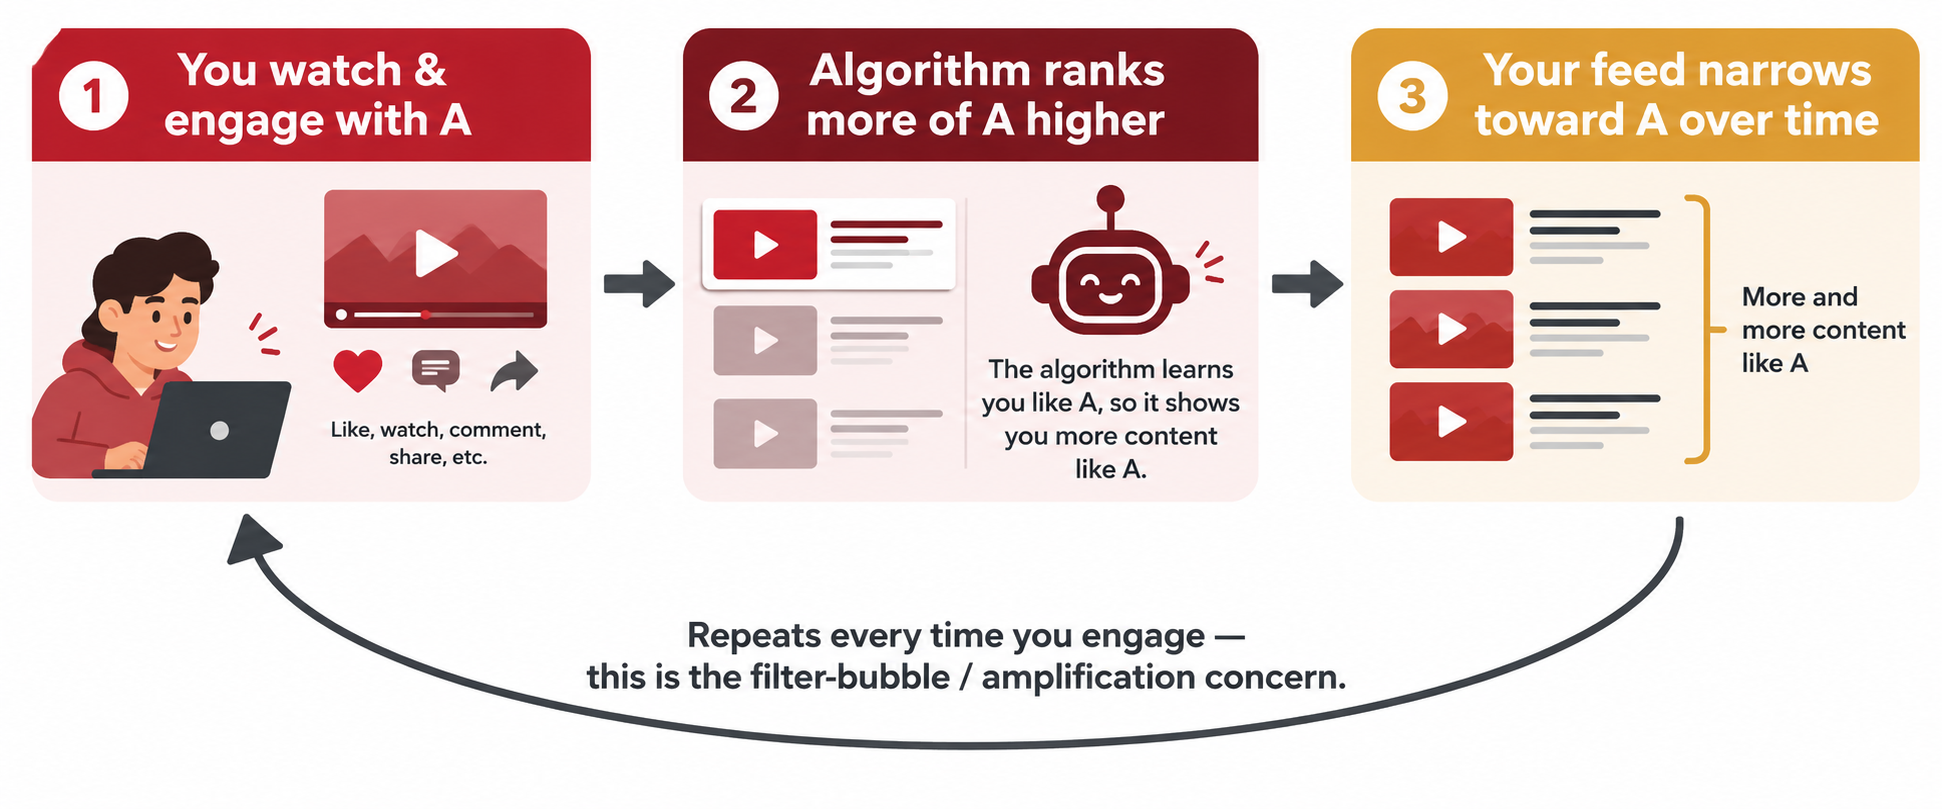
\includegraphics[width=0.68\textwidth]{figs/biased_rec.png}}

\vspace{2pt}
\begin{itemize}
\item Recommenders are optimised for engagement (watch time, clicks),
  not for your wellbeing or a balanced information diet
\item The same feedback loop that makes recommendations good also makes
  bias self-reinforcing: filter bubbles, algorithmic amplification
\item \textbf{The explore/exploit trade-off:} always showing what you
  already like (\emph{exploit}) entrenches the bias; trying something
  different (\emph{explore}) is how the system learns (Week 8 multi-armed bandits)
% \item \textbf{Ties to Ethics (Week 7)} and \textbf{RL (Week 9):}
%   fairness/accountability, and the explore/exploit trade-off
%   (multi-armed bandits); both apply daily, not just to ``AI'' in the
%   abstract
\end{itemize}

\end{frame}
%%%%%%%%%%%%%%%%%%%%%%%%%%%%%%%%%%%%%%%%%%%%%%%%%%%%%%%%%%%%%%%%%%%%%%
\begin{frame}[fragile]
\frametitle{Correlation Isn't Causation}
\framesubtitle{AI for X \textperiodcentered\ Epidemiology}

\centerline{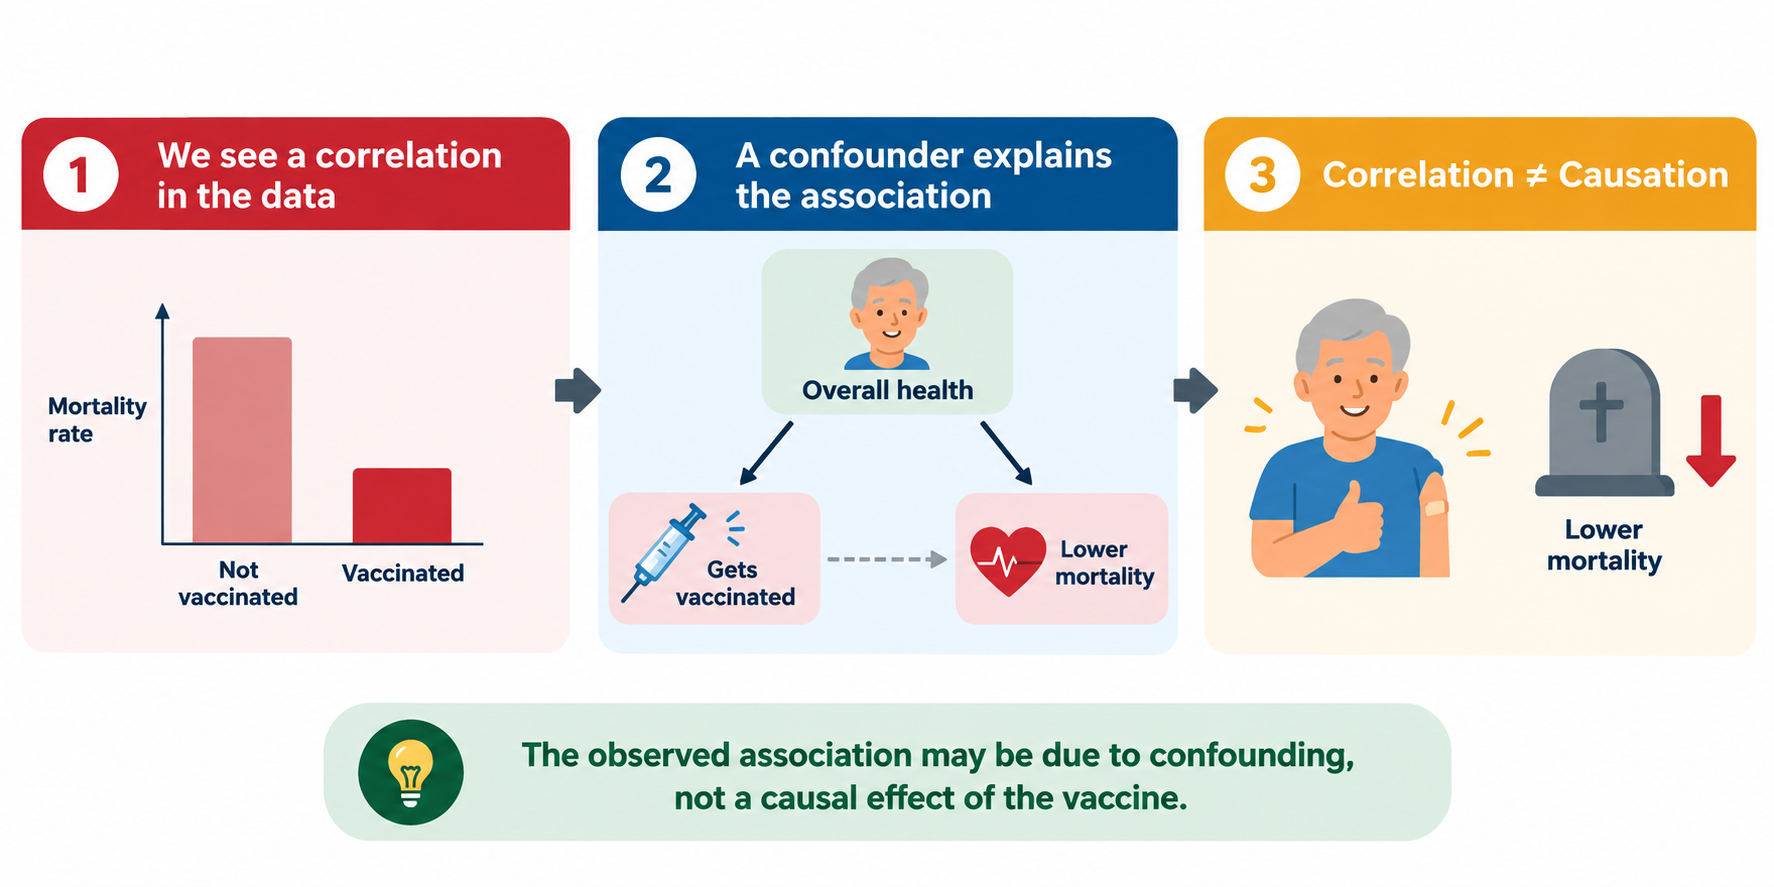
\includegraphics[width=0.8\textwidth]{figs/causal.png}}

\vspace{8pt}
\begin{itemize}
\item Do healthier people simply choose to get
  vaccinated more often?
\item Machine learning finds patterns; causal inference asks whether a
  pattern reflects a real effect
\item This distinction, correlation vs.\ causation, is the subject of
  Week 8
\end{itemize}

\end{frame}
%%%%%%%%%%%%%%%%%%%%%%%%%%%%%%%%%%%%%%%%%%%%%%%%%%%%%%%%%%%%%%%%%%%%%%
\begin{frame}[fragile]
\frametitle{Beating the World Champion at Go}
\framesubtitle{AI for X \textperiodcentered\ Reinforcement Learning}

\begin{columns}[T]
\begin{column}{0.42\textwidth}
\centerline{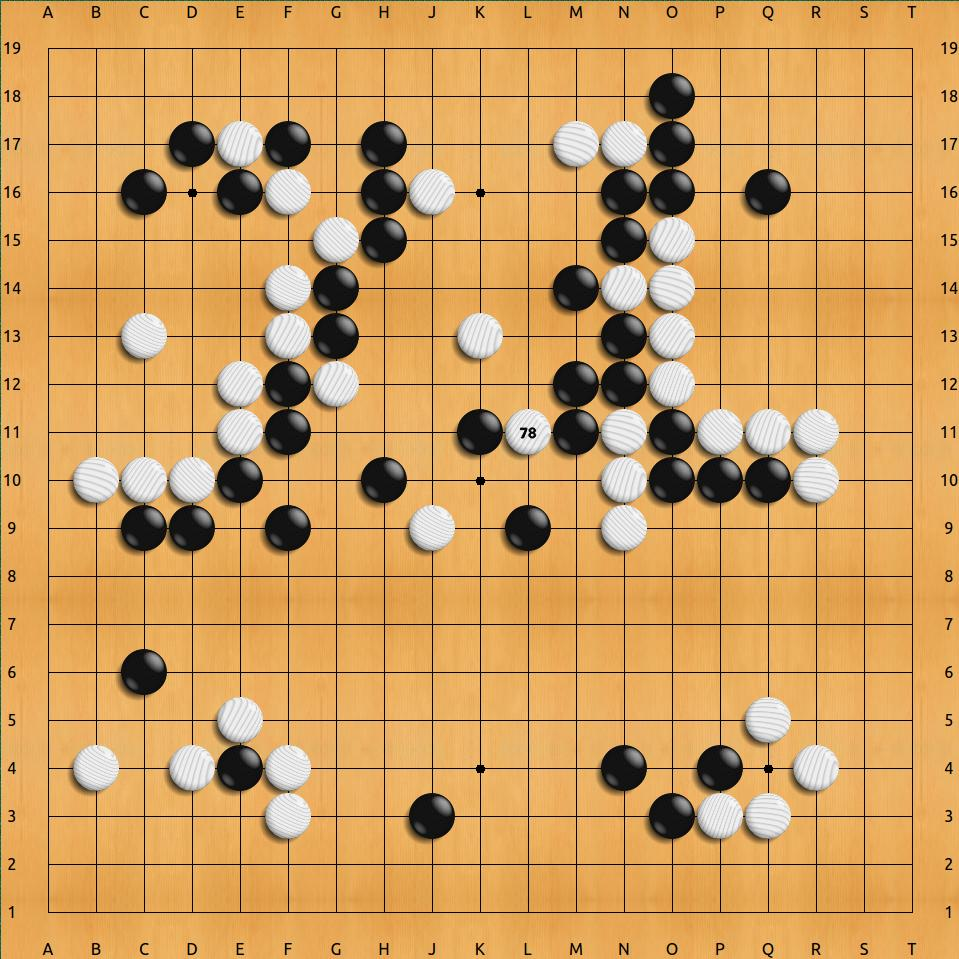
\includegraphics[width=\textwidth]{figs/alphago.jpg}}
\end{column}
\begin{column}{0.56\textwidth}
\begin{itemize}
\item \textbf{The game of Go has more possible positions than atoms in
  the universe}, too many to search exhaustively
\item AlphaGo (DeepMind, 2016) beat world champion Lee Sedol 4--1
\item \textbf{Under the hood:} trained by playing millions of games
  against itself, learning from the reward of winning or losing 
  (week 9: reinforcement learning)
\item Same family of ideas behind game-playing agents, robotics, and RLHF
  fine-tuning of LLMs
\end{itemize}
\end{column}
\end{columns}

\vspace{8pt}
{\footnotesize Image: board position after AlphaGo's ``divine move'' 78
vs.\ Lee Sedol (2016). Axd, Wikimedia Commons, CC BY-SA 4.0.}

\end{frame}
%%%%%%%%%%%%%%%%%%%%%%%%%%%%%%%%%%%%%%%%%%%%%%%%%%%%%%%%%%%%%%%%%%%%%%
\begin{frame}[fragile]
\frametitle{Teaching Machines to See}
\framesubtitle{AI for X \textperiodcentered\ Computer Vision}

\begin{columns}[T]
\begin{column}{0.5\textwidth}
\centerline{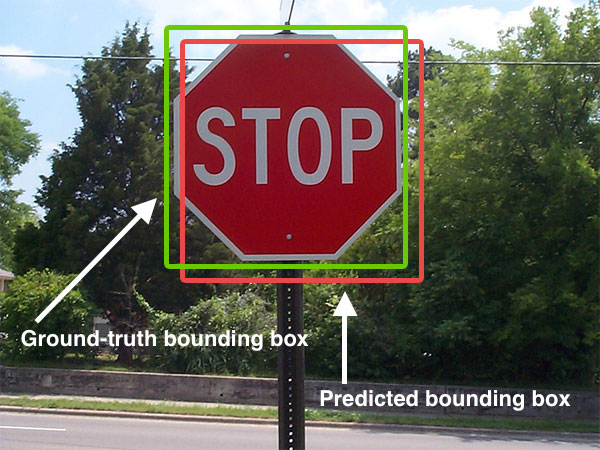
\includegraphics[width=\textwidth]{figs/cv_detection.jpg}}
\end{column}
\begin{column}{0.48\textwidth}
\begin{itemize}
\item Task: locate and label objects in an image (detection), or classify
  a whole image (classification)
\item \textbf{Under the hood:} Convolutional Neural Networks (CNNs)
  trained via supervised learning on millions of labelled images
\item Applications: self-driving cars, quality control, satellite imagery
% \item You'll build CNNs in Weeks 3 and 10
\end{itemize}
\end{column}
\end{columns}

\vspace{8pt}
{\footnotesize Image: Adrian Rosebrock, PyImageSearch, Wikimedia Commons,
CC BY-SA 4.0.}

\end{frame}
%%%%%%%%%%%%%%%%%%%%%%%%%%%%%%%%%%%%%%%%%%%%%%%%%%%%%%%%%%%%%%%%%%%%%%
\begin{frame}[fragile]
\frametitle{Spotting Endangered Species From Millions of Photos}
\framesubtitle{AI for X \textperiodcentered\ Computer Vision, continued}

\begin{columns}[T]
\begin{column}{0.5\textwidth}
\centerline{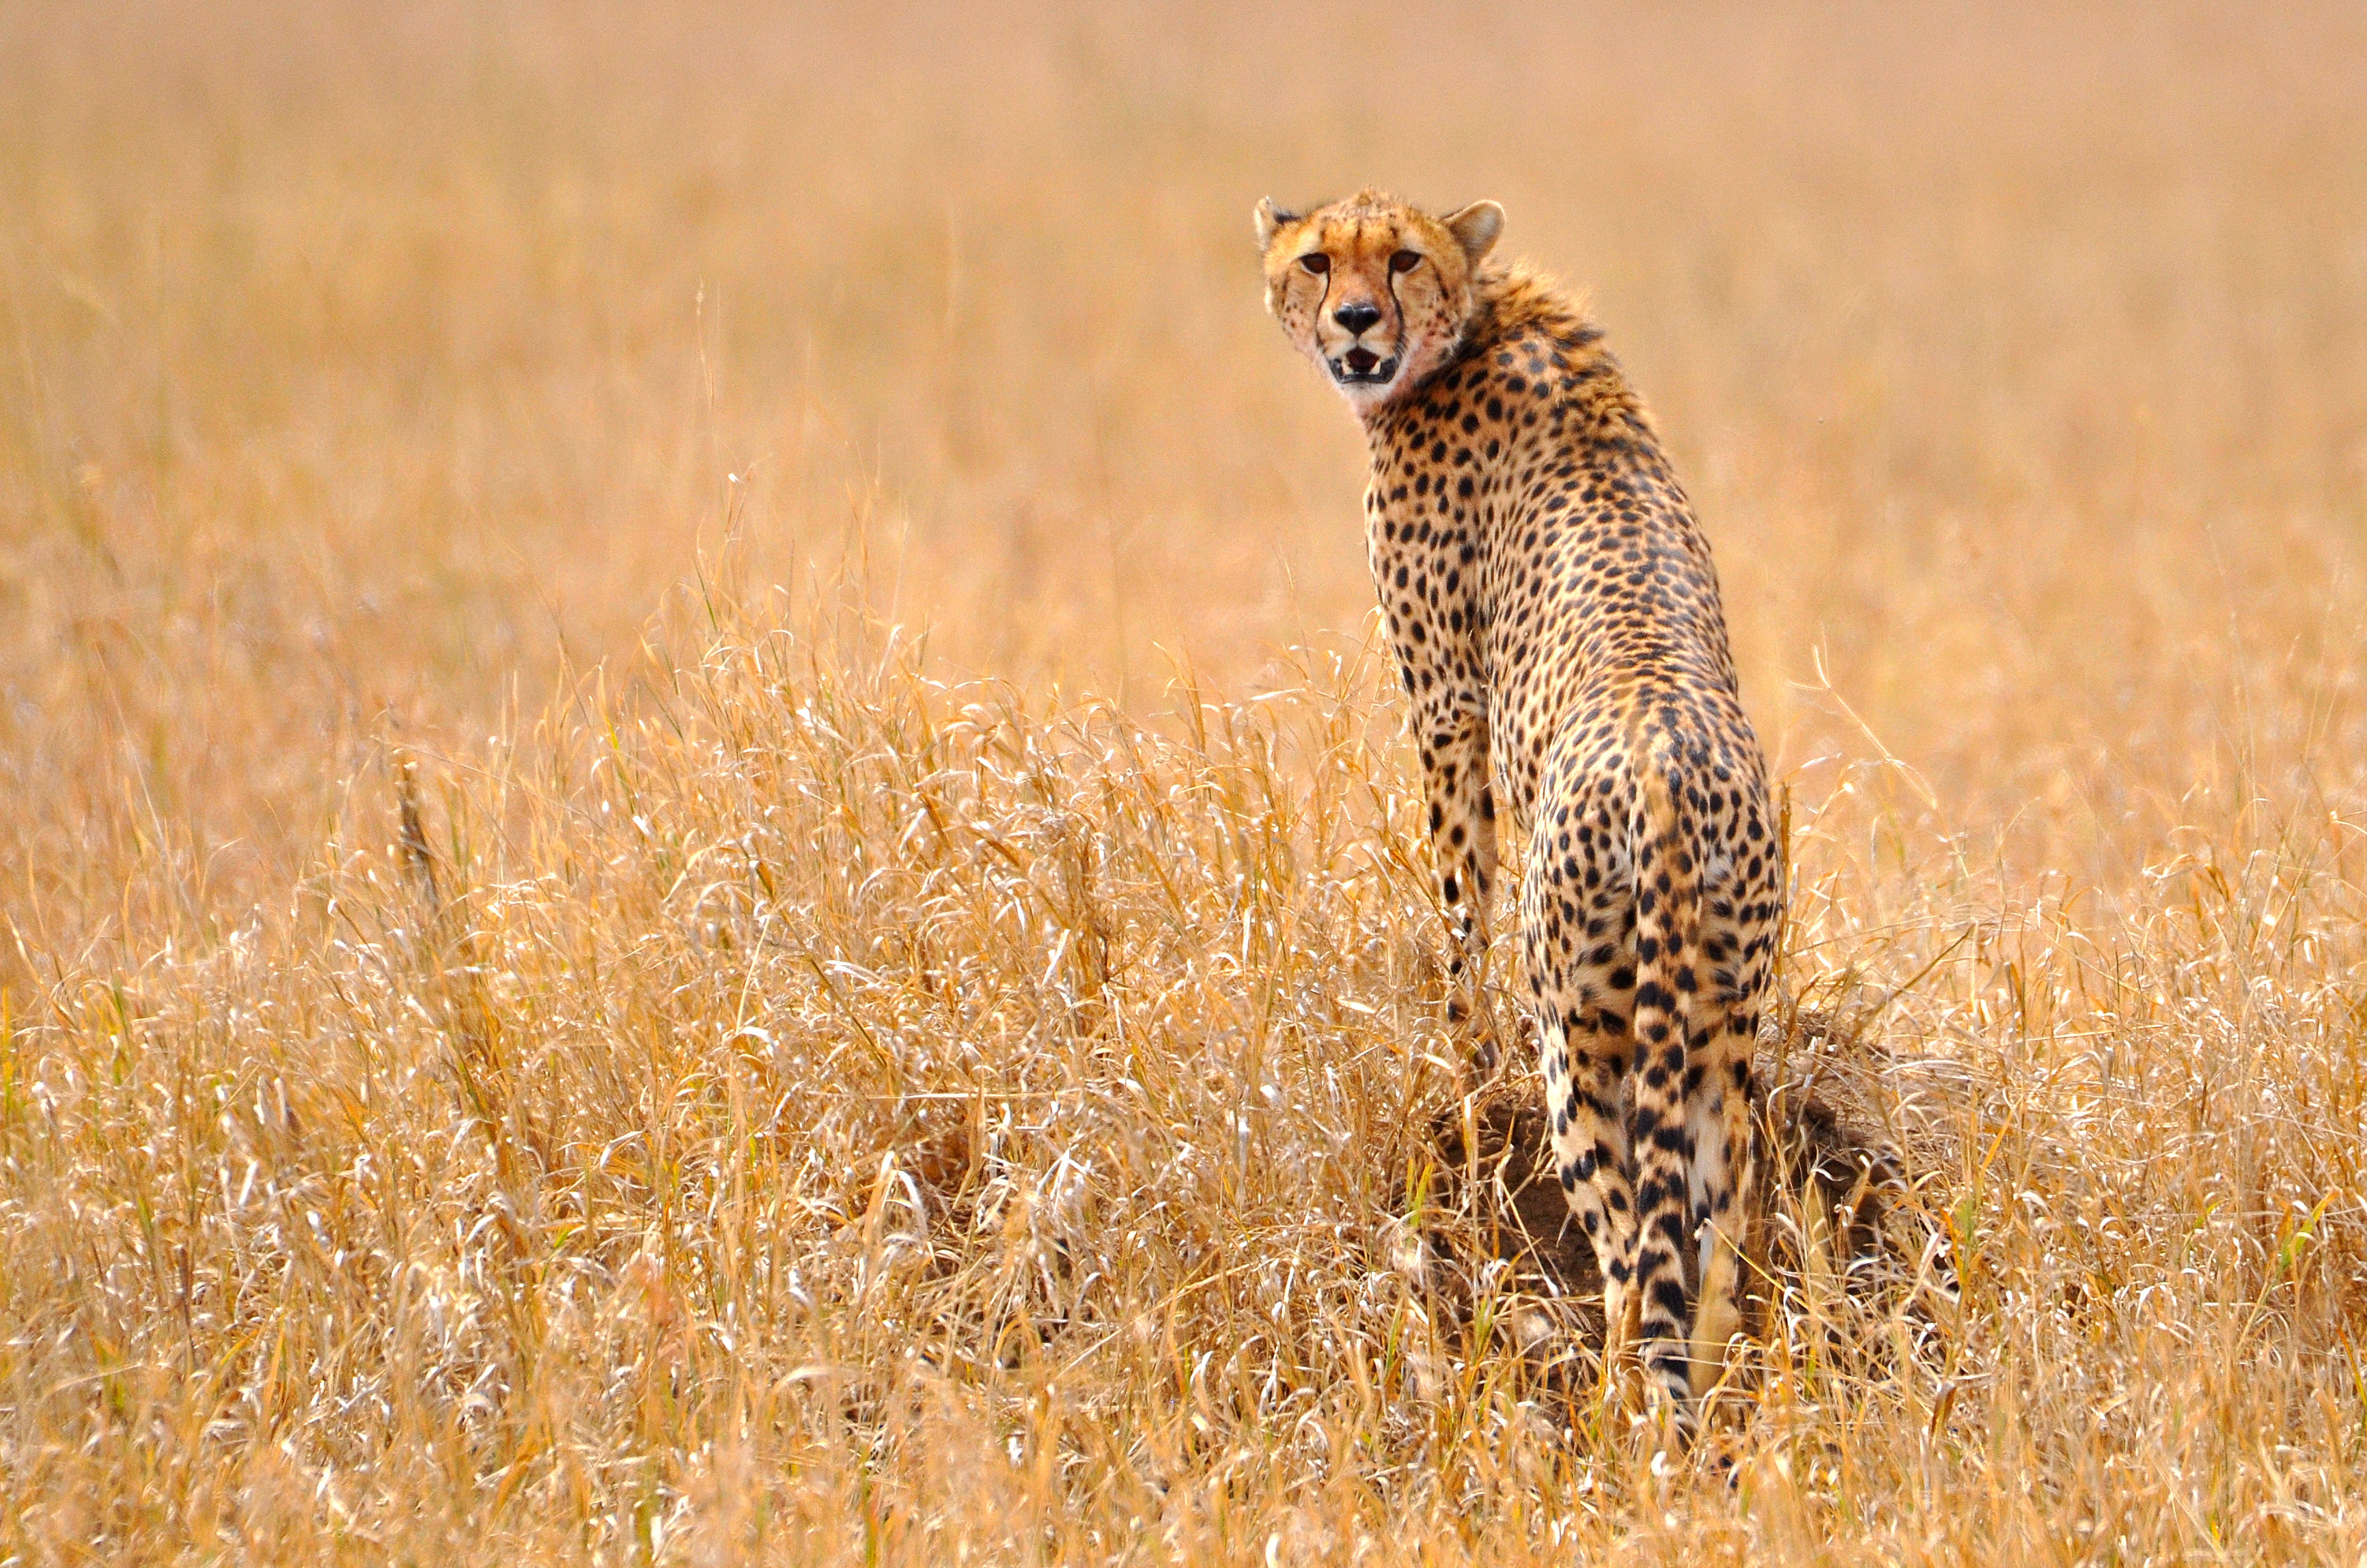
\includegraphics[width=\textwidth]{figs/wildlife.jpg}}
\end{column}
\begin{column}{0.48\textwidth}
\begin{itemize}
\item Camera traps and drones collect far more wildlife photos than
  ecologists can label by hand
\item \textbf{Under the hood:} CNNs classify species (and count
  individuals) automatically, at a scale no human team could match
\item Used by conservation projects (e.g.\ Wildlife Insights, Snapshot
  Serengeti) to track endangered populations
% \item Same technique as the stop-sign example, a different, very
%   worthwhile use of it
\end{itemize}
\end{column}
\end{columns}

\vspace{8pt}
{\footnotesize Image: cheetah, Serengeti National Park. Tobi 87, Wikimedia
Commons, CC BY-SA 3.0.}

\end{frame}
%%%%%%%%%%%%%%%%%%%%%%%%%%%%%%%%%%%%%%%%%%%%%%%%%%%%%%%%%%%%%%%%%%%%%%
\begin{frame}[fragile]
\frametitle{A Second Opinion From a Neural Network}
\framesubtitle{AI for X \textperiodcentered\ Healthcare}

\begin{columns}[T]
\begin{column}{0.4\textwidth}
\centerline{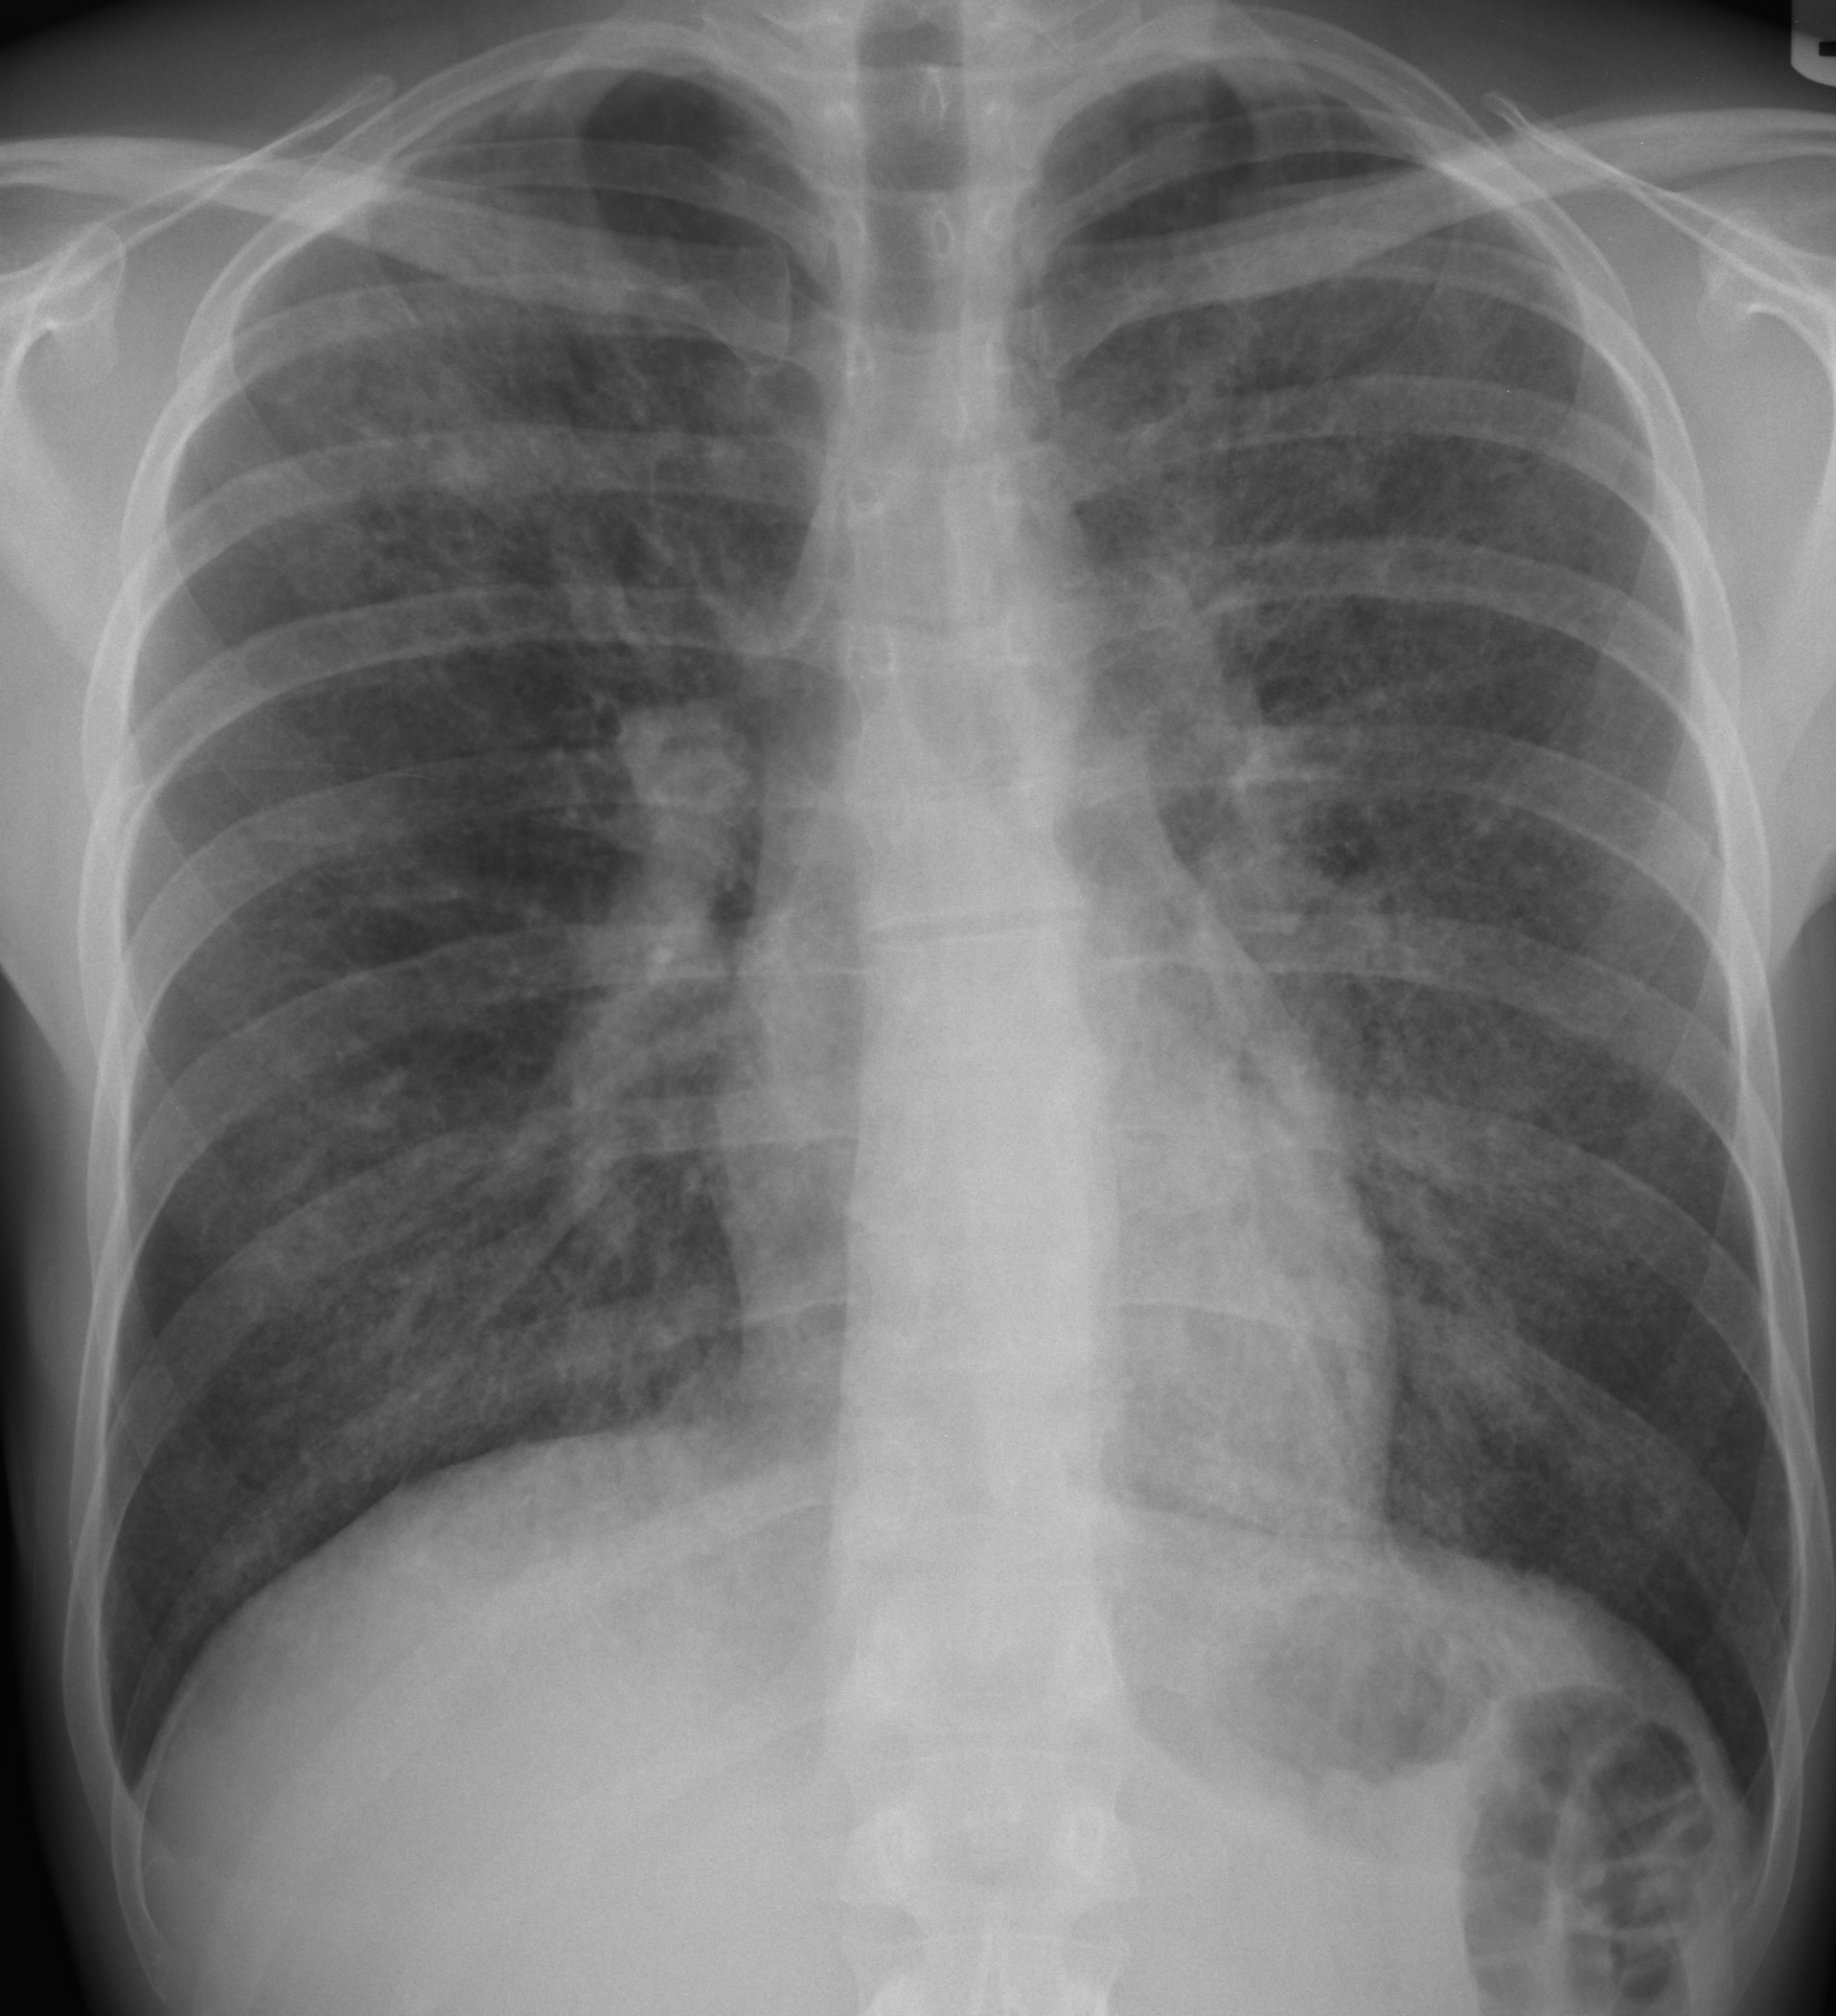
\includegraphics[width=\textwidth]{figs/healthcare_xray.jpg}}
\end{column}
\begin{column}{0.57\textwidth}
\begin{itemize}
\item CNNs trained on labelled X-rays can flag disease (e.g.\ pneumonia)
  at radiologist-level accuracy
\item \textbf{Example:} CheXNet, a 121-layer CNN trained on 100,000+
  chest X-rays (Stanford, 2017)
\item These are decision-support tools, not replacements for clinicians
\item \textbf{Ties to Trustworthy AI (Week 11):} safety, fairness and
  accountability matter enormously here
\end{itemize}
\end{column}
\end{columns}

\vspace{8pt}
{\footnotesize Image: chest X-ray showing \emph{Pneumocystis} pneumonia.
Samir, Wikimedia Commons, public domain. Method: Rajpurkar et al.,
CheXNet (2017).}

\end{frame}
%%%%%%%%%%%%%%%%%%%%%%%%%%%%%%%%%%%%%%%%%%%%%%%%%%%%%%%%%%%%%%%%%%%%%%
\begin{frame}[fragile]
\frametitle{The Landscape of AI Applications}
% \framesubtitle{Recap}

\begin{center}
\resizebox{0.98\textwidth}{!}{%
\begin{tabular}{ccccc}
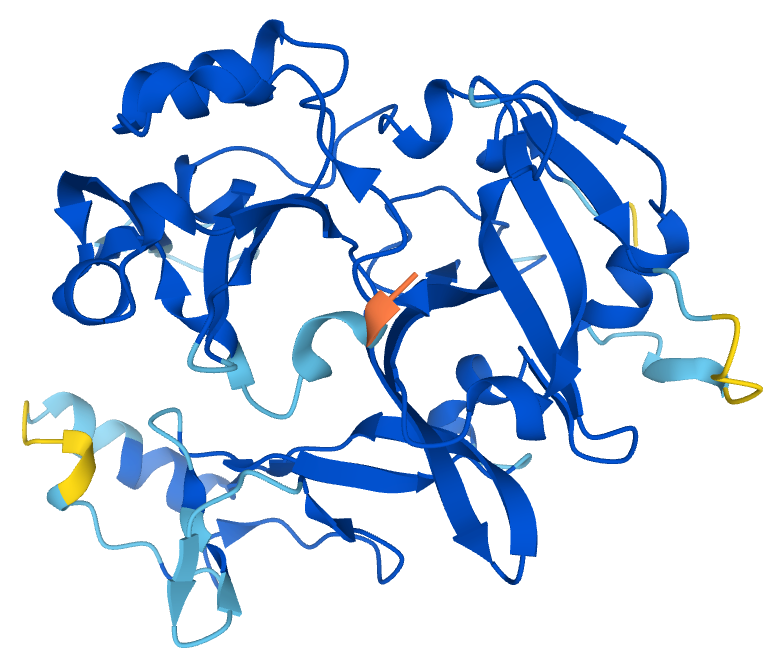
\includegraphics[height=2.1cm]{figs/protein.png} &
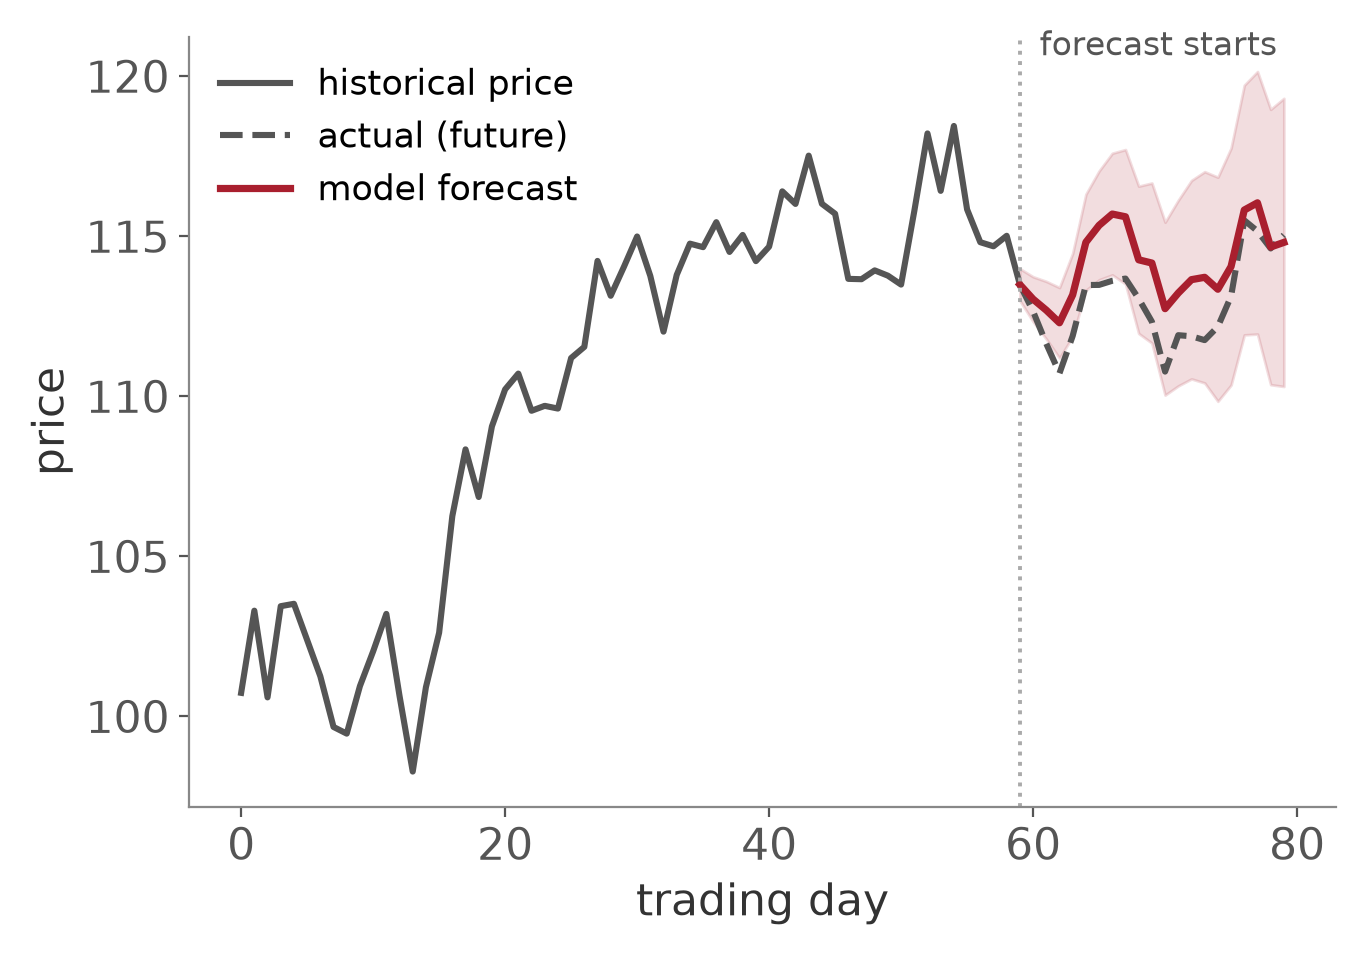
\includegraphics[height=2.1cm]{figs/finance_chart.png} &
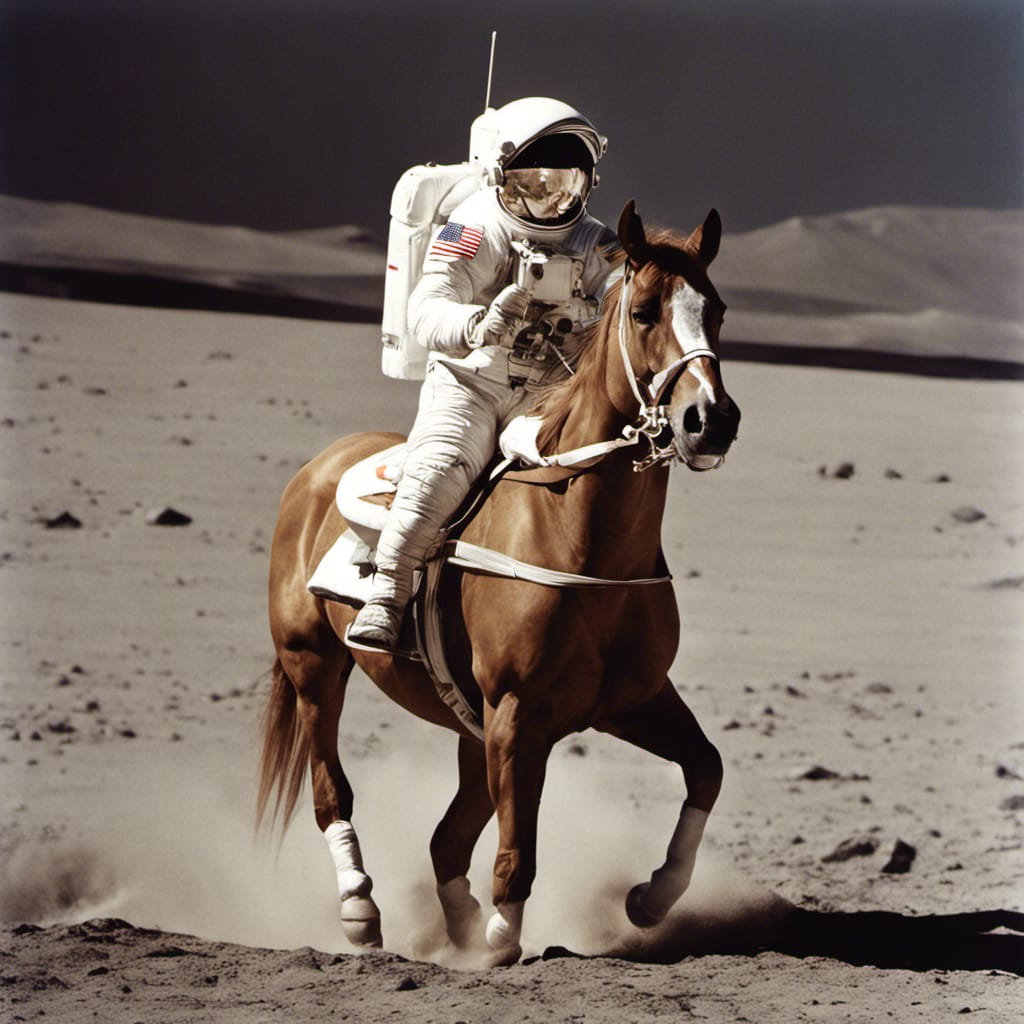
\includegraphics[height=2.1cm]{figs/genai.jpg} &

\includegraphics[height=2.1cm]{figs/tiktok_phone.png} &
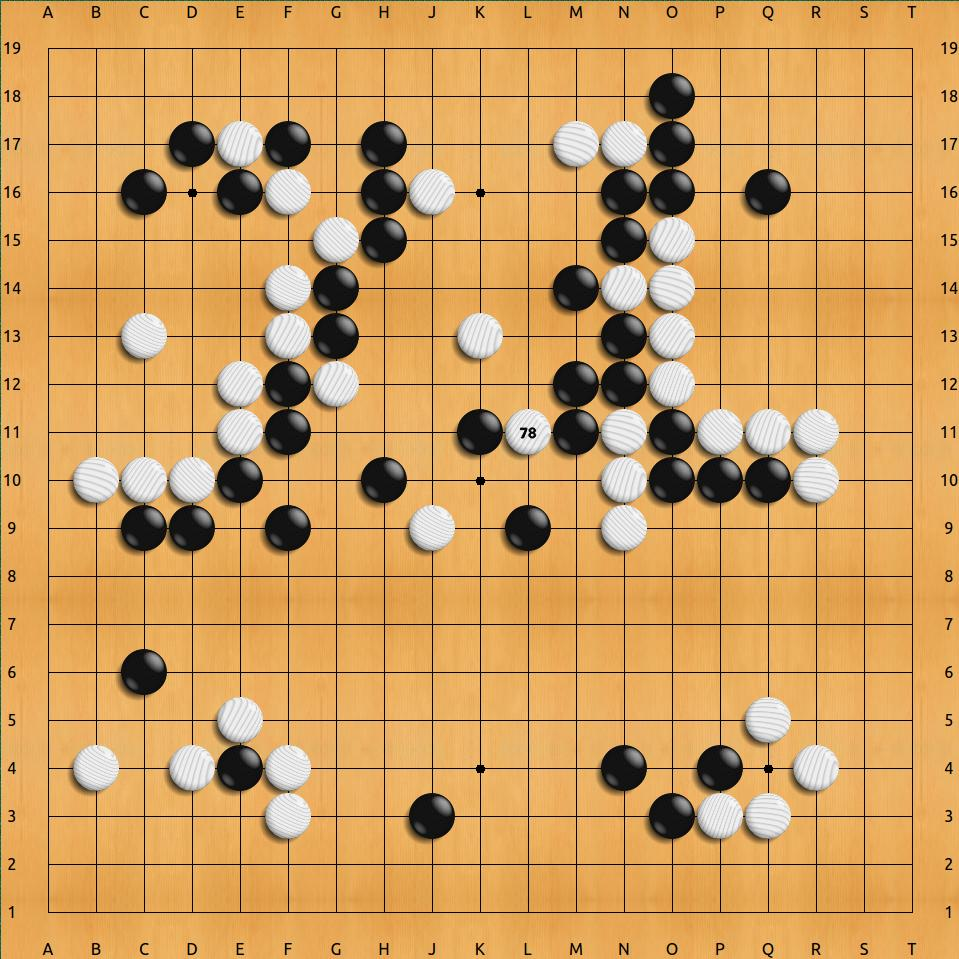
\includegraphics[height=2.1cm]{figs/alphago.jpg} \\
{\small Science} & {\small Finance} & {\small Generative AI} &
{\small Recommenders} & {\small Game playing} \\[8pt]
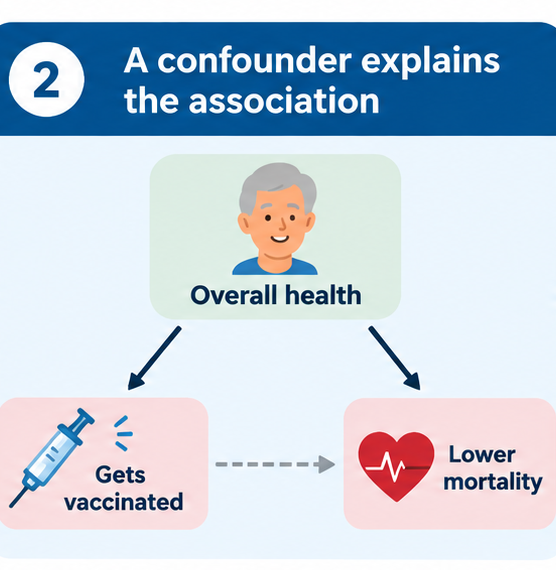
\includegraphics[height=2.1cm]{figs/causal_middle.png} &
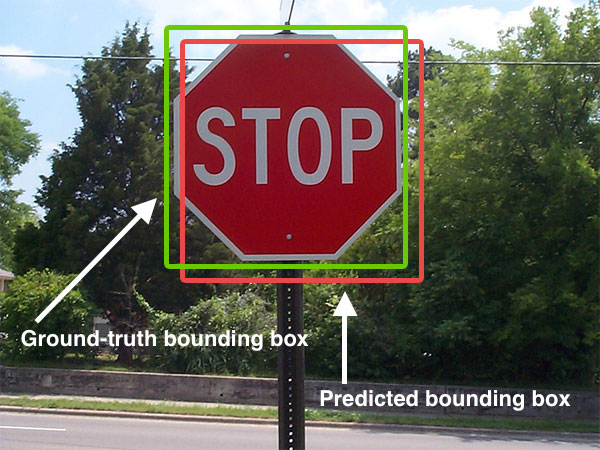
\includegraphics[height=2.1cm]{figs/cv_detection.jpg} &
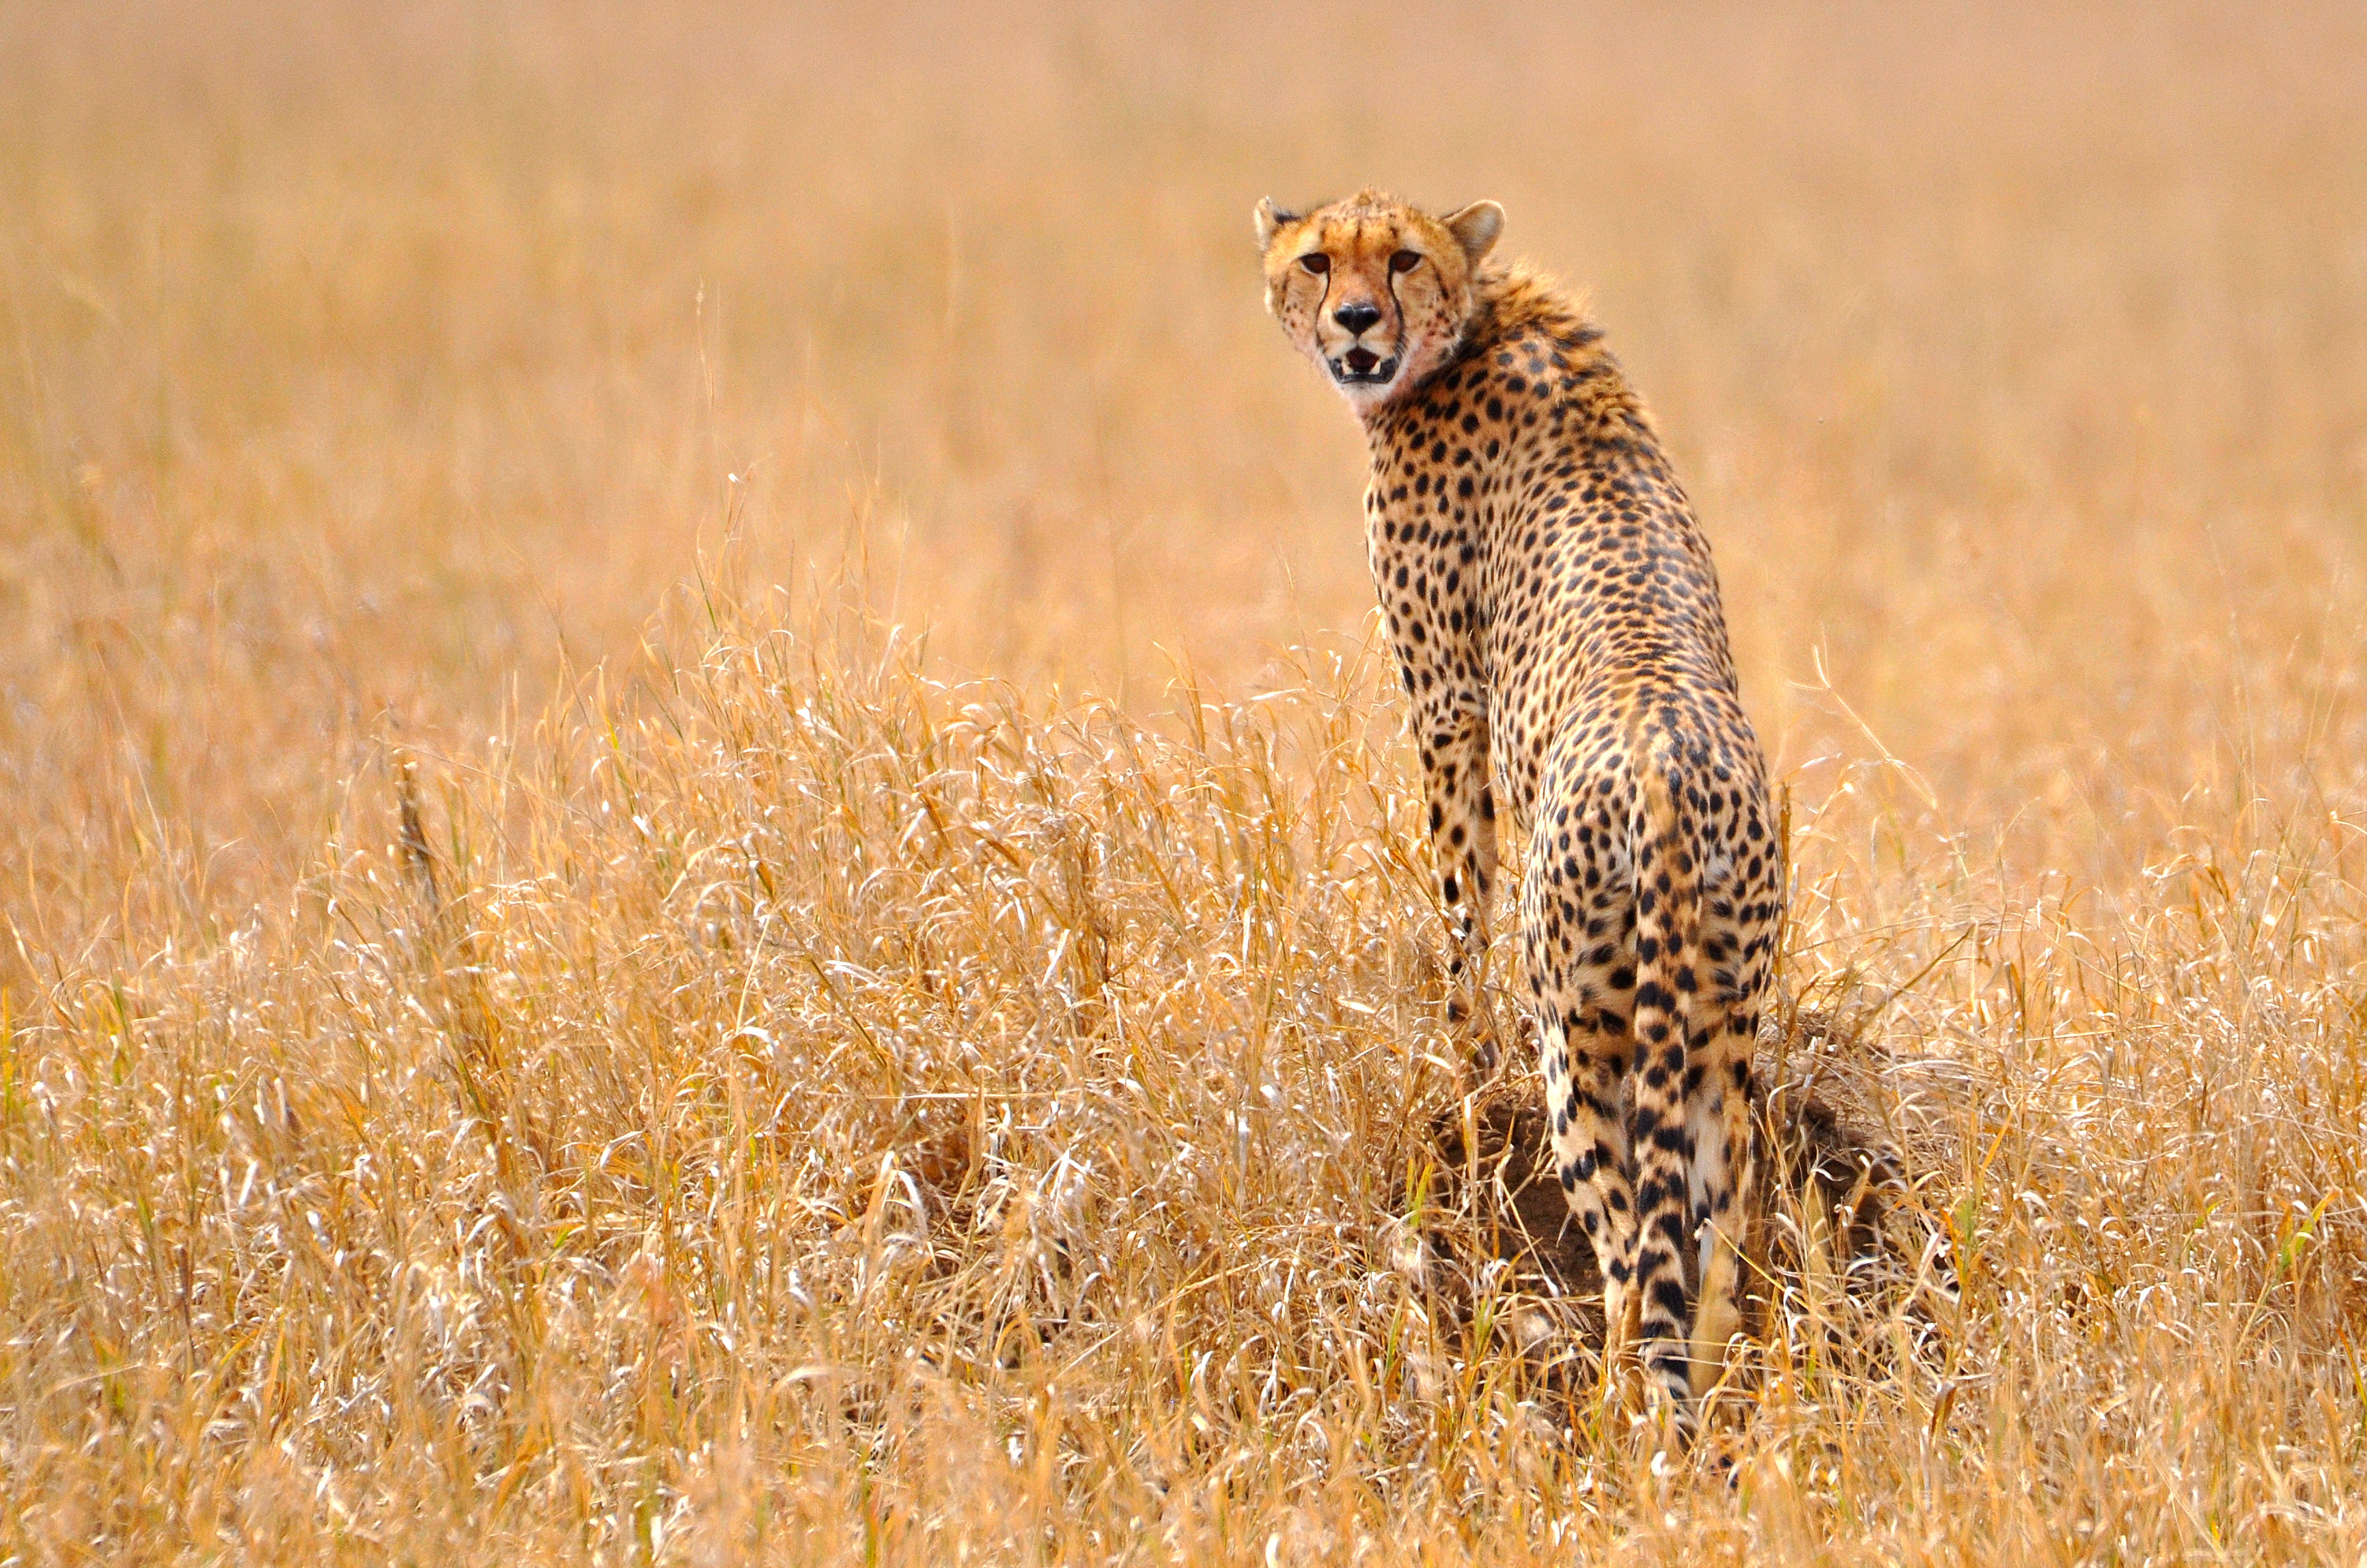
\includegraphics[height=2.1cm]{figs/wildlife.jpg} &
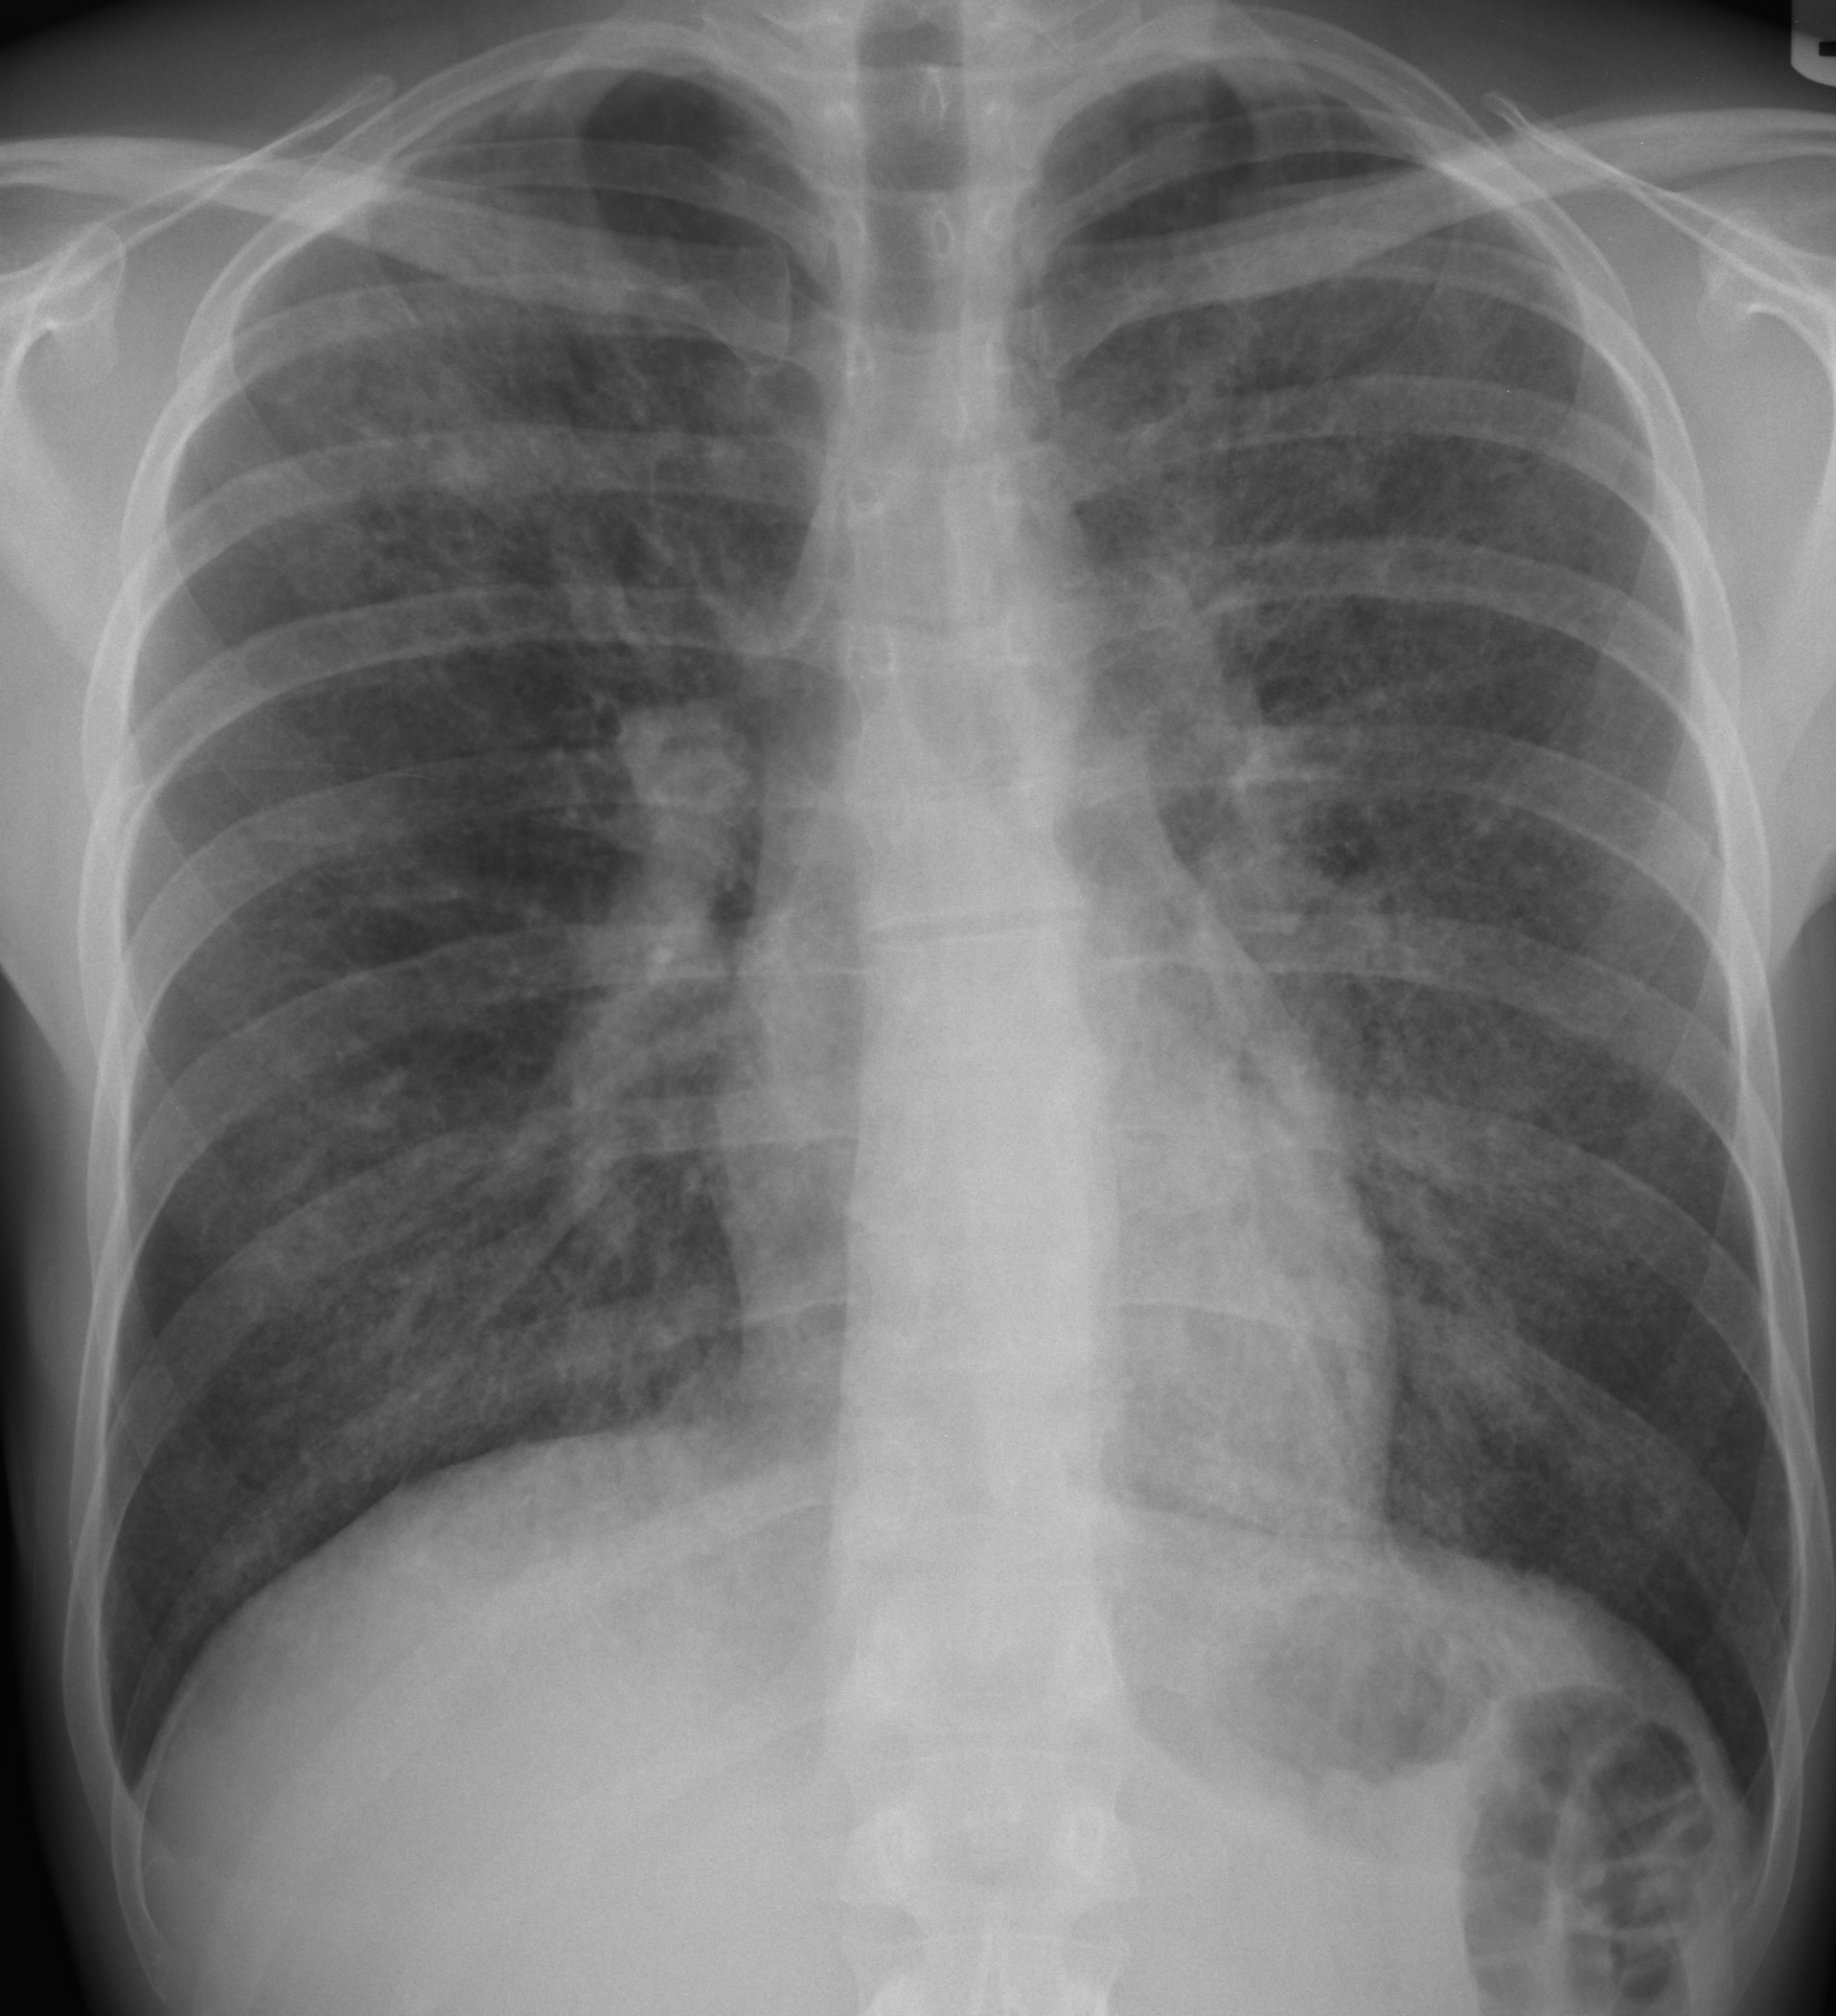
\includegraphics[height=2.1cm]{figs/healthcare_xray.jpg} &

\includegraphics[height=0.9cm]{figs/tool_logo1.png} \\
{\small Epidemiology} & {\small Computer vision} & {\small Conservation} &
{\small Healthcare} & {\small Everyday AI tools}
\end{tabular}}
\end{center}

\vspace{10pt}
% \begin{itemize}
% \item[$\Rightarrow$] That's the tour: eleven applications you now know a bit
%   more about, each built on ideas this unit will teach you, week by week.
% \end{itemize}

\end{frame}
%%%%%%%%%%%%%%%%%%%%%%%%%%%%%%%%%%%%%%%%%%%%%%%%%%%%%%%%%%%%%%%%%%%%%%
\end{document}
